\documentclass[11pt,a4paper]{article}
\usepackage{fontspec}
\setmainfont{TeX Gyre Pagella}
\newfontfamily\headfont{Inter}[UprightFont=*-ExtraBold,BoldFont=*-ExtraBold,Extension=.otf,Path=/usr/share/fonts/opentype/inter/]
\usepackage[a4paper,margin=2.3cm]{geometry}
\usepackage{graphicx,booktabs,float,caption,array,xcolor,longtable}
\usepackage{xurl}
\usepackage[hidelinks]{hyperref}
\usepackage{titlesec}
\usepackage[round]{natbib}
\usepackage{setspace}
\setstretch{1.05}
\renewcommand{\topfraction}{0.9}
\renewcommand{\bottomfraction}{0.8}
\renewcommand{\textfraction}{0.1}
\renewcommand{\floatpagefraction}{0.75}
\setlength{\parindent}{0pt}
\setlength{\parskip}{0.55em}
\titleformat{\section}{\headfont\Large}{\thesection}{0.8em}{}
\titleformat{\subsection}{\headfont\large}{\thesubsection}{0.8em}{}
\captionsetup{font=small,labelfont=bf}
\urlstyle{same}
\hypersetup{pdftitle={Where the World's Music Comes From},pdfauthor={Tristan Hotham}}

\begin{document}
\begin{center}
{\Large\bfseries Where the World's Music Comes From\par}
\vspace{0.4em}
{\large The birthplaces of 291,579 musicians and the home towns of bands in Wikidata,\\by city, genre, decade and gender\par}
\vspace{1.2em}
{\large Tristan Hotham\par}
\vspace{0.3em}
{\small Independent researcher\\
ORCID: 0000-0003-4931-9349\\
DOI: https://doi.org/10.5281/zenodo.23850287\par}
\vspace{0.8em}
2026
\end{center}

\begin{quote}
\small
\begin{center}\textbf{Abstract}\end{center}
Where are musicians born, and where do bands begin? I use Wikidata, the open knowledge base behind Wikipedia, to map everyone it records with an occupation that is musician or any of its subclasses (478,552 people) and every musical group (115,219). 291,579 musicians (61\%) have a birth country and 283,424 a birthplace with coordinates; 29,489 groups have a place of formation with coordinates. Grouping places into city areas, New York (6,124 musicians), London (4,627), Paris (4,466) and Vienna (4,102) lead for births, and Los Angeles (1,454), New York and London for bands. Composers born before 1900 were 88\% European, pop, rock and metal musicians born since 1940 only 48\%. Many genres have a clear home town: Kingston holds 23\% of reggae acts, Seoul 52\% of K-pop acts, Rio de Janeiro 57\% of samba acts, and Nashville's acts are 13.0 times as likely as the world's to be country. Finland has 84.8 metal bands per million people. Women are 25.4\% of musicians with a recorded gender, rising from 8.1\% of those born before 1800 to 41.9\% of those born in the 1990s, with large differences by kind of musician. Coverage is very uneven: a birth country is recorded for 99.8\% of notable musicians but 46\% of those with at most one sitelink, and a formation place for 27\% of groups. The atlas maps the open record of music, not every musician.

\textbf{Keywords:} musicians; bands; music geography; music scenes; genres; gender; Wikidata; open data; mapping
\end{quote}

\section{Introduction}
Music has always had places. Histories of Western art music are organised around courts, churches and conservatories in a handful of central European cities; histories of popular music around scenes, from New Orleans and Memphis to Liverpool, Kingston, Seattle and Seoul \citep{connell, bennett}. Geographers have long mapped where musicians come from, starting with the birthplaces of American country and rock musicians \citep{carney}. A simple question cuts across these traditions: where were the world's musicians born, and where did its bands form?

Wikidata \citep{wikidata} offers a way to ask it at a scale no single history can. It records hundreds of thousands of people with musical occupations, many with a place and date of birth, and more than a hundred thousand musical groups, some with a place and date of formation, and it links both to genres. Studies of notable people's birth and death places have shown how much structure such data hold, and how much they reflect the biases of their sources \citep{schich}. This paper maps musicians' birthplaces and bands' formation places by city, country, kind of musician, genre and decade, measures where each genre is concentrated, and tracks the share of women. It pairs the analysis with an interactive atlas (\url{https://maps.tristanhotham.com/music-birthplaces/}).

The contribution is descriptive. Wikidata is not a census of musicians. Its coverage depends on which library catalogues and music databases have been imported and which people have Wikipedia articles, and its records of gender follow those of Wikipedia, where women are known to be under-represented \citep{wagner}. I report coverage alongside every result.

\section{Data}
\textbf{Musicians.} A query through the QLever SPARQL endpoint \citep{qlever}, retrieved in 2026, returned every human (P31 Q5) with an occupation (P106) that is musician (Q639669) or a subclass of it, with English label, occupation, place of birth (P19), that place's English label, coordinates (P625) and country (P17), date of birth (P569), sex or gender (P21) and number of sitelinks. The export was paged to avoid a time-out; it has 818,669 rows (one per combination of values) for 478,552 people, the same number as a separate count of the set. Six lines lacked a line break and were repaired. 534 occupations appear, from composer, singer and pianist to organist, rapper, kobzar and bertsolari. 63,026 people have no English label.

\textbf{Groups.} A second query returned every item that is an instance of musical group (Q215380) or a subclass, with type, location of formation (P740) and its coordinates and country, inception (P571), dissolution (P576), country of origin (P495) and sitelinks: 118,971 rows for 115,219 groups. Groups include rock bands, idol groups and duos, and also 4,273 choirs, orchestras and ensembles, identified from their type labels.

\textbf{Genres.} Two further queries returned the genres (P136) of musicians and groups and the English labels of the 3,743 genres used.

\textbf{Geography.} Natural Earth \citep{naturalearth} countries (1:10m for assigning points, 1:50m for display), land and populated places, with population estimates. All Wikidata content is CC0 and Natural Earth is public domain.

\begin{table}[tbp]\centering\small\caption{From query to data.}\label{tab:pipe}\begin{tabular}{p{10.5cm}r}\toprule Step & Count\\\midrule
Rows returned by the musician query & 818,669\\
Musicians & 478,552\\
\quad with a birthplace & 292,146\\
\quad with a birth country & 291,579\\
\quad with a birthplace point (on the map) & 283,424\\
\quad\quad of which in a city area & 181,847\\
\quad with a year of birth & 384,245\\
\quad with a recorded gender & 458,411\\
\quad with a genre & 110,334\\
\quad notable (20+ sitelinks) & 10,946\\
Musical groups & 115,219\\
\quad with a country & 90,469\\
\quad with a formation place & 31,190\\
\quad with a formation point (on the map) & 29,489\\
\quad with a year of formation & 44,057\\
\quad with a genre & 65,023\\
\bottomrule\end{tabular}\end{table}

\section{Methods}
\subsection{Places and countries}
A musician's birthplace is the first place of birth in the result (2,848 have more than one) and its point is that place's coordinates. 6,968 birthplaces are themselves countries or former states (for example `Austrian Empire'); these give a country but no point. The birth country is the present-day Natural Earth country that the point falls in, else the place's Wikidata country matched to Natural Earth by Wikidata identifier, with a hand-made table of successors for former states. Where both are known they agree for 99\% of musicians. A group's place is its location of formation, and its country that of the place, else its country of origin.

\subsection{City areas and per-head rates}
Wikidata often records a district (Brooklyn, Hollywood, a Paris arrondissement) rather than a city. I assign each point to the nearest Natural Earth populated place of 200,000 people or more within 25 km, merging any such place within 25 km of a larger one, so that Liverpool and Manchester stay apart but Brooklyn counts with New York. 64\% of musicians' points fall in one of 1,725 city areas. Per-head rates divide by Natural Earth's present-day population: a rough guide, since most of these musicians were born when cities were smaller and in different proportion to each other.

\subsection{Kinds of musician and genre families}
I grouped the occupations into eight families (composers and arrangers, singers, instrumentalists, rappers and MCs, DJs and producers, conductors and bandleaders, songwriters, and other musicians, mostly the generic `musician') and the genres into thirteen families plus `other' (classical and opera; rock and punk; metal; pop; K-pop, J-pop and East Asian pop; hip hop; R\&B, soul, blues and gospel; jazz; electronic and dance; country; Latin; reggae, Caribbean and African popular; folk and traditional), using ordered rules on English labels checked against the most-used values. Both mappings are published with the data. A person or group belongs to every family of any of its occupations or genres; 160,553 people are in more than one occupation family. Genre shares are among genre-tagged acts only (23\% of musicians and 56\% of groups have a genre).

\subsection{Home towns of genres}
For each of 34 named genres I count the acts (musicians born and groups formed) in each city area and report the city with most and its share of all such acts with a point. For the genre families I also compute a location quotient: a family's share of a city's genre-tagged acts divided by its share of all genre-tagged acts, for cities with 25 or more acts in the family and 40 or more tagged acts.

\subsection{Decades, gender and notability}
Musicians are placed in the decade of their birth (earliest valid year of P569, 800 to 2020; before 1800 pooled) and groups in the decade of their formation. Women and trans women are counted as women and men and trans men as men; 685 musicians have another gender recorded. Shares are among musicians with a recorded gender (96\%). Notable musicians and groups are those with 20 or more sitelinks (10,946 musicians, 1,948 groups), a measure of attention on Wikipedia and its sister projects, not of musical standing.

\section{Results}
\subsection{The map}
Figure~\ref{fig:map} shows all 283,424 birthplace points in hexagons. They are densest in central and western Europe, the eastern United States, Japan and Korea, and sparse across Africa and Central Asia. Europe accounts for 60\% of musicians with a birth country, North America 18\%, Asia 14\%, South America 5.0\%, Africa 2.6\% and Oceania 0.9\%. The maps of bands, of women and of notable musicians (Figure~\ref{fig:small}) differ in instructive ways: bands are concentrated in North America, western Europe and Japan, and notable musicians in the United States and Britain.

\begin{figure}[tbp]\centering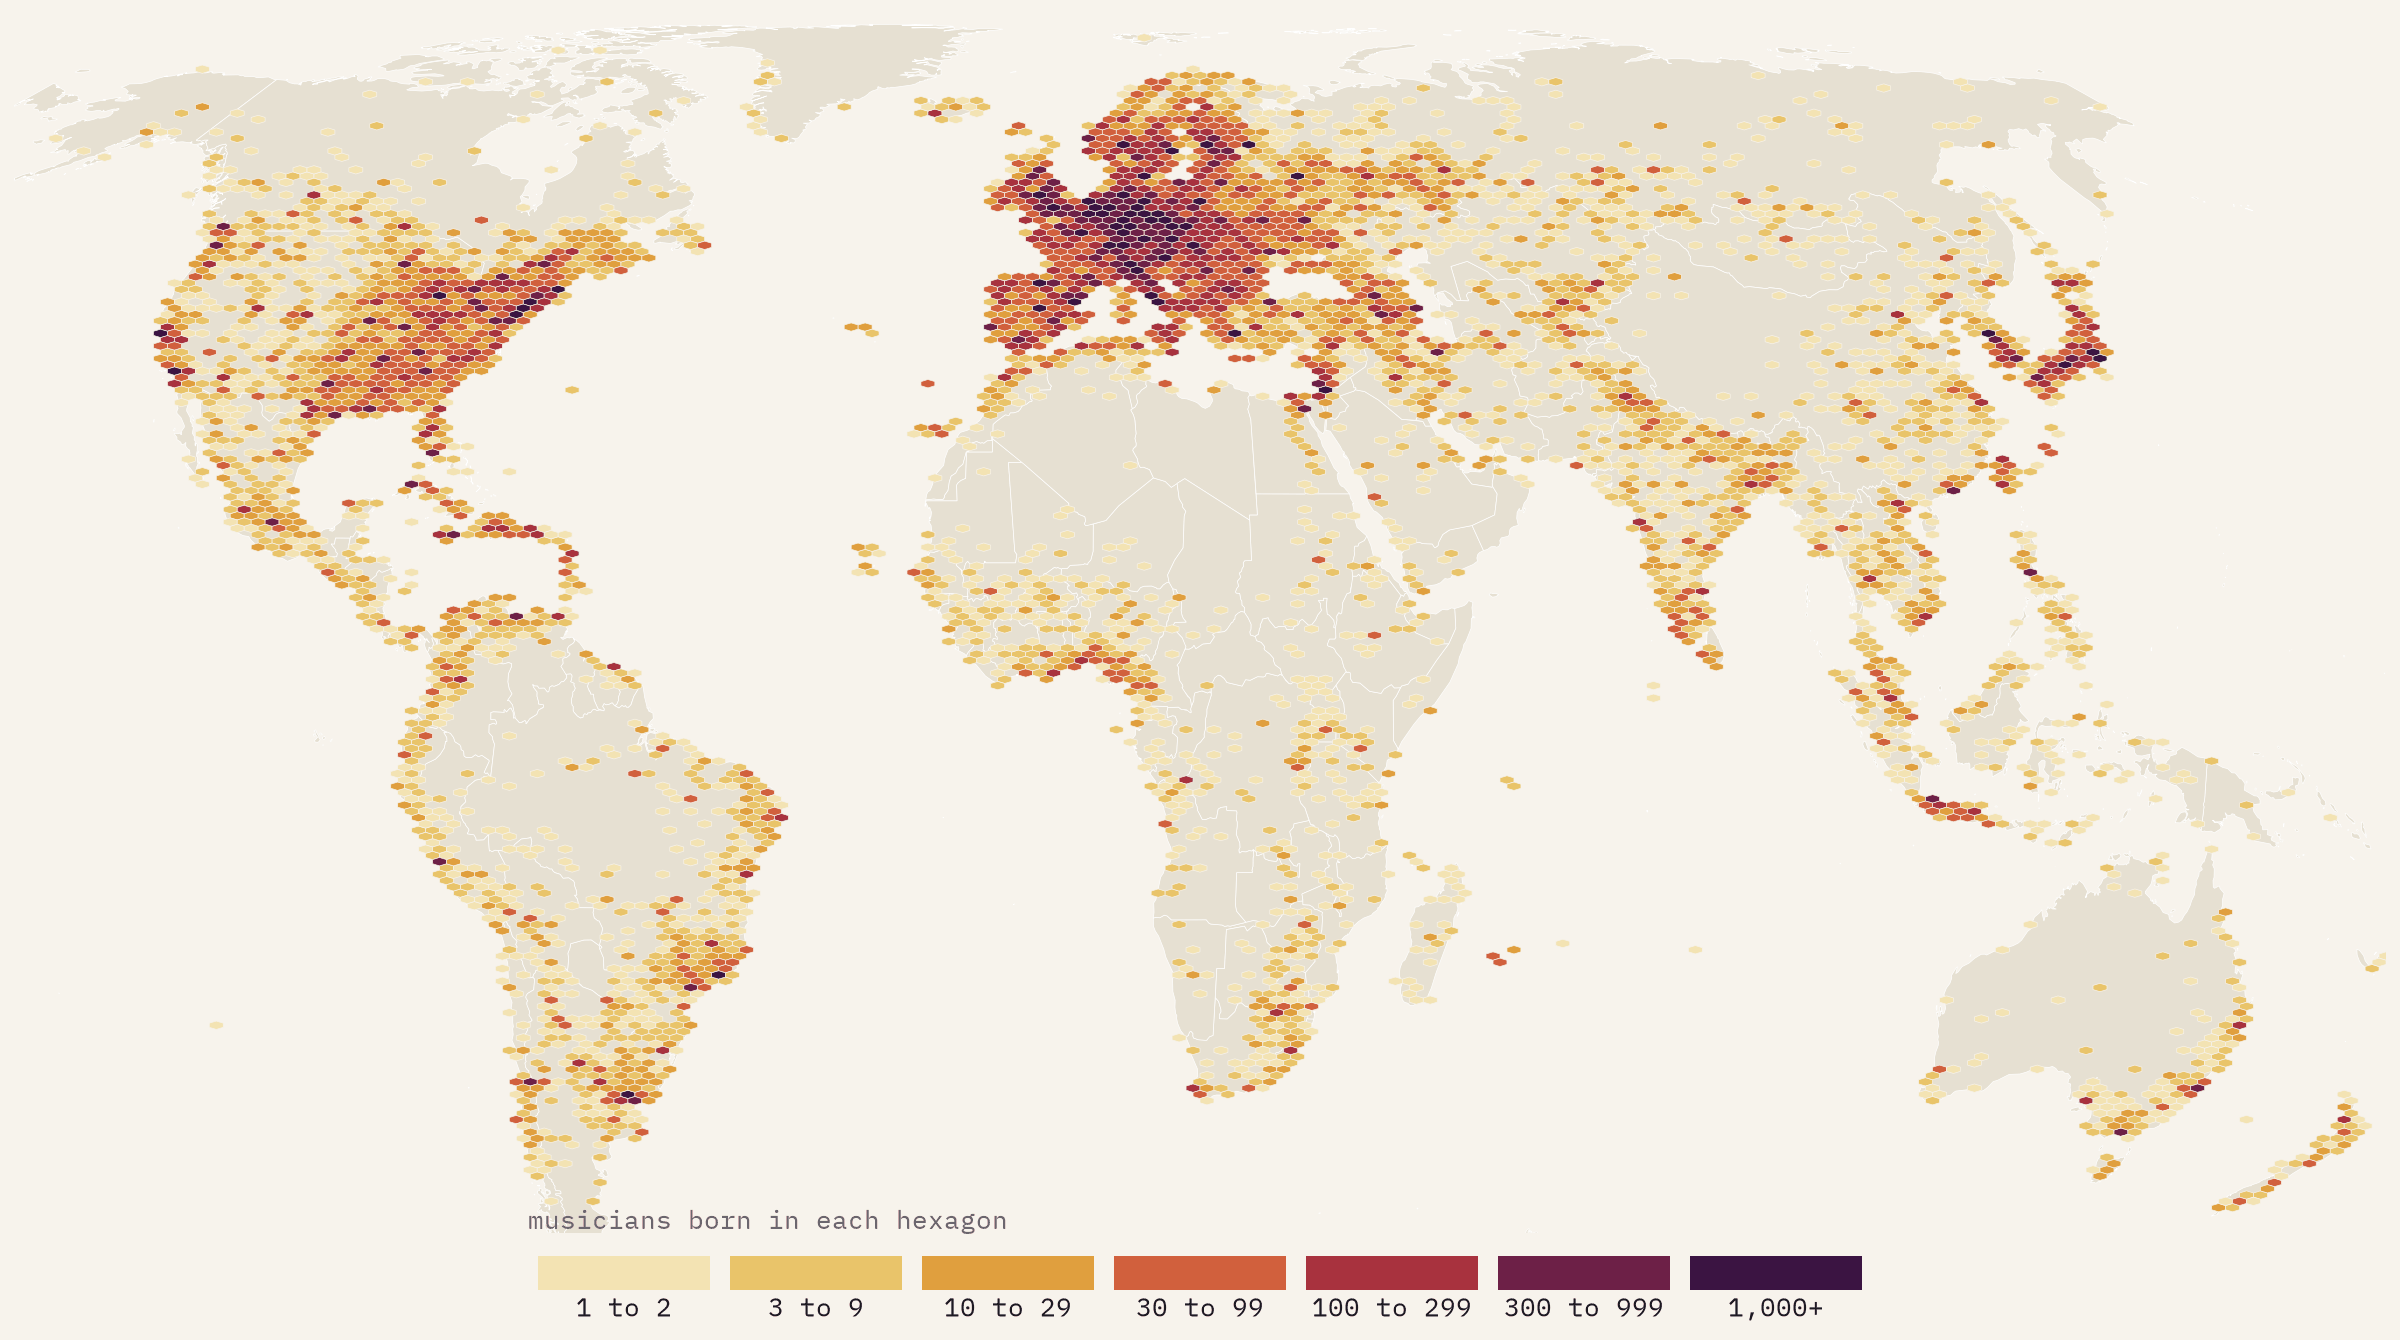
\includegraphics[width=\textwidth]{f_map.png}
\caption{Birthplaces of 283,424 musicians in Wikidata, counted in hexagons (Equal Earth projection).}\label{fig:map}\end{figure}

\begin{figure}[tbp]\centering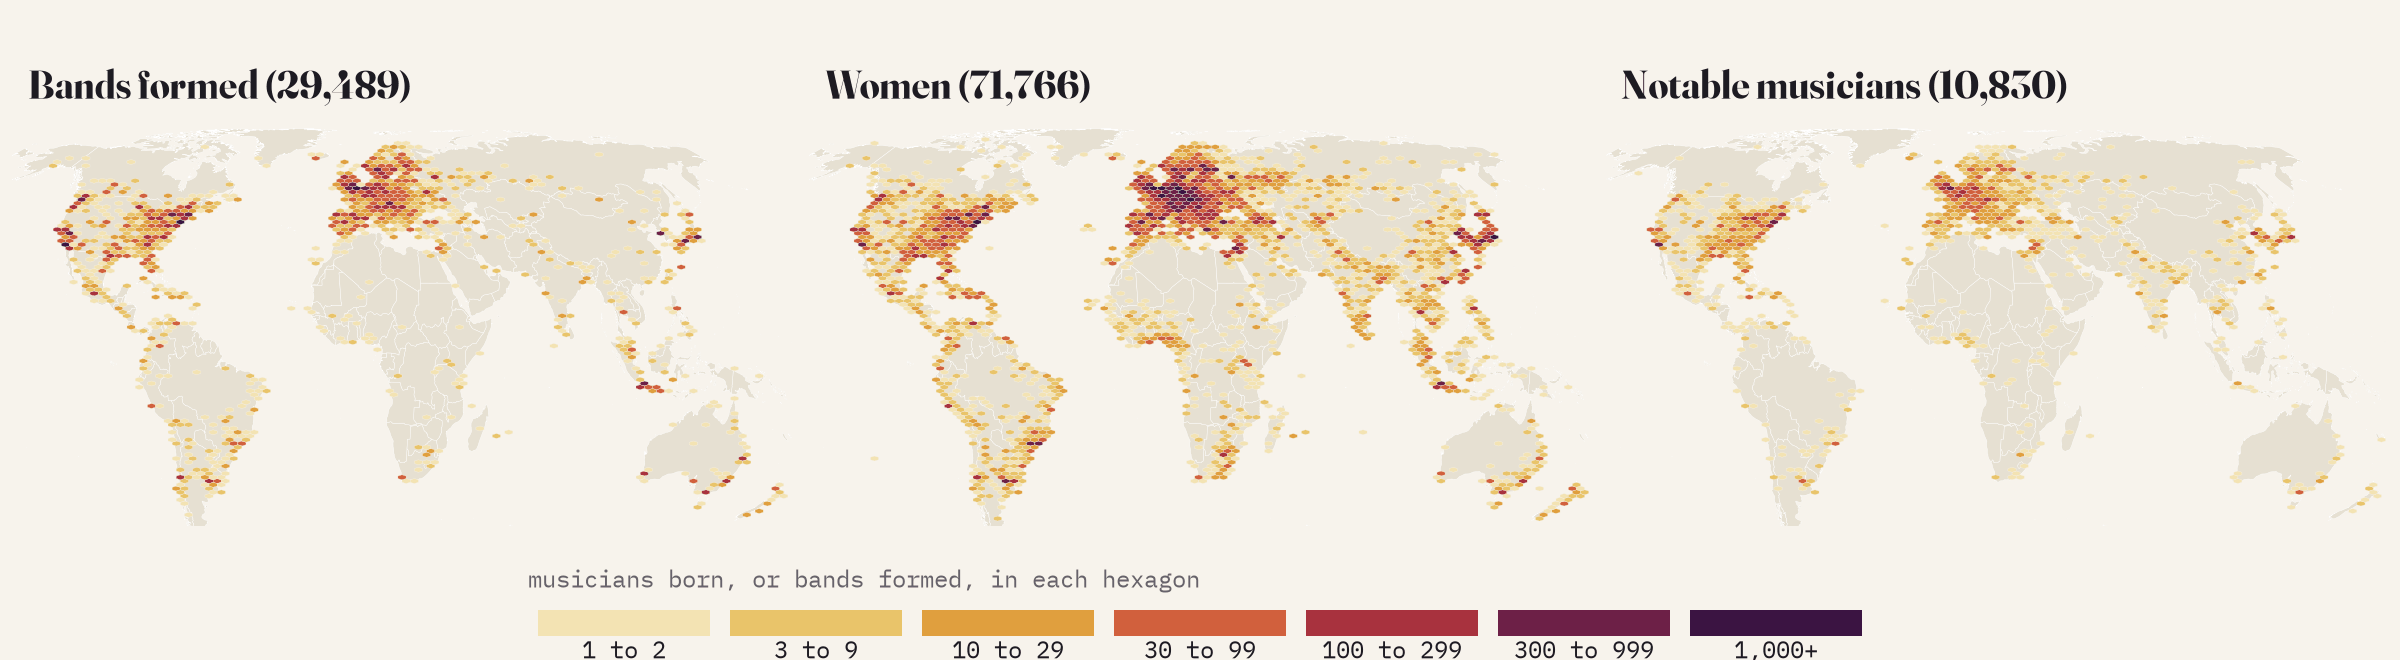
\includegraphics[width=\textwidth]{f_small_maps.png}
\caption{Where bands formed (left), where women musicians were born (centre) and where notable musicians, with 20 or more sitelinks, were born (right).}\label{fig:small}\end{figure}

\subsection{Cities}
As a single Wikidata place, Vienna is the most common birthplace (3,784), ahead of New York City (2,948) and London (2,792). Grouped into city areas (Figure~\ref{fig:cities}, Table~\ref{tab:cities}), New York leads with 6,124 musicians, then London, Paris, Vienna, Tokyo, Berlin and Prague; the ten largest areas hold 12\% of all points. Per head of present population, the leaders are smaller central European cities, Tallinn, Prague, Brno and Erfurt, with more than 230 musicians per 100,000 residents; among cities of a million or more, Prague (246.1) and Vienna (170.9) lead, against New York's 32.2 and Tokyo's 9.2. Bands have a different geography: Los Angeles has most (1,454), then New York, London, Tokyo and San Francisco, and per head Ljubljana, Bergen, Malmö and Oslo.

\begin{figure}[tbp]\centering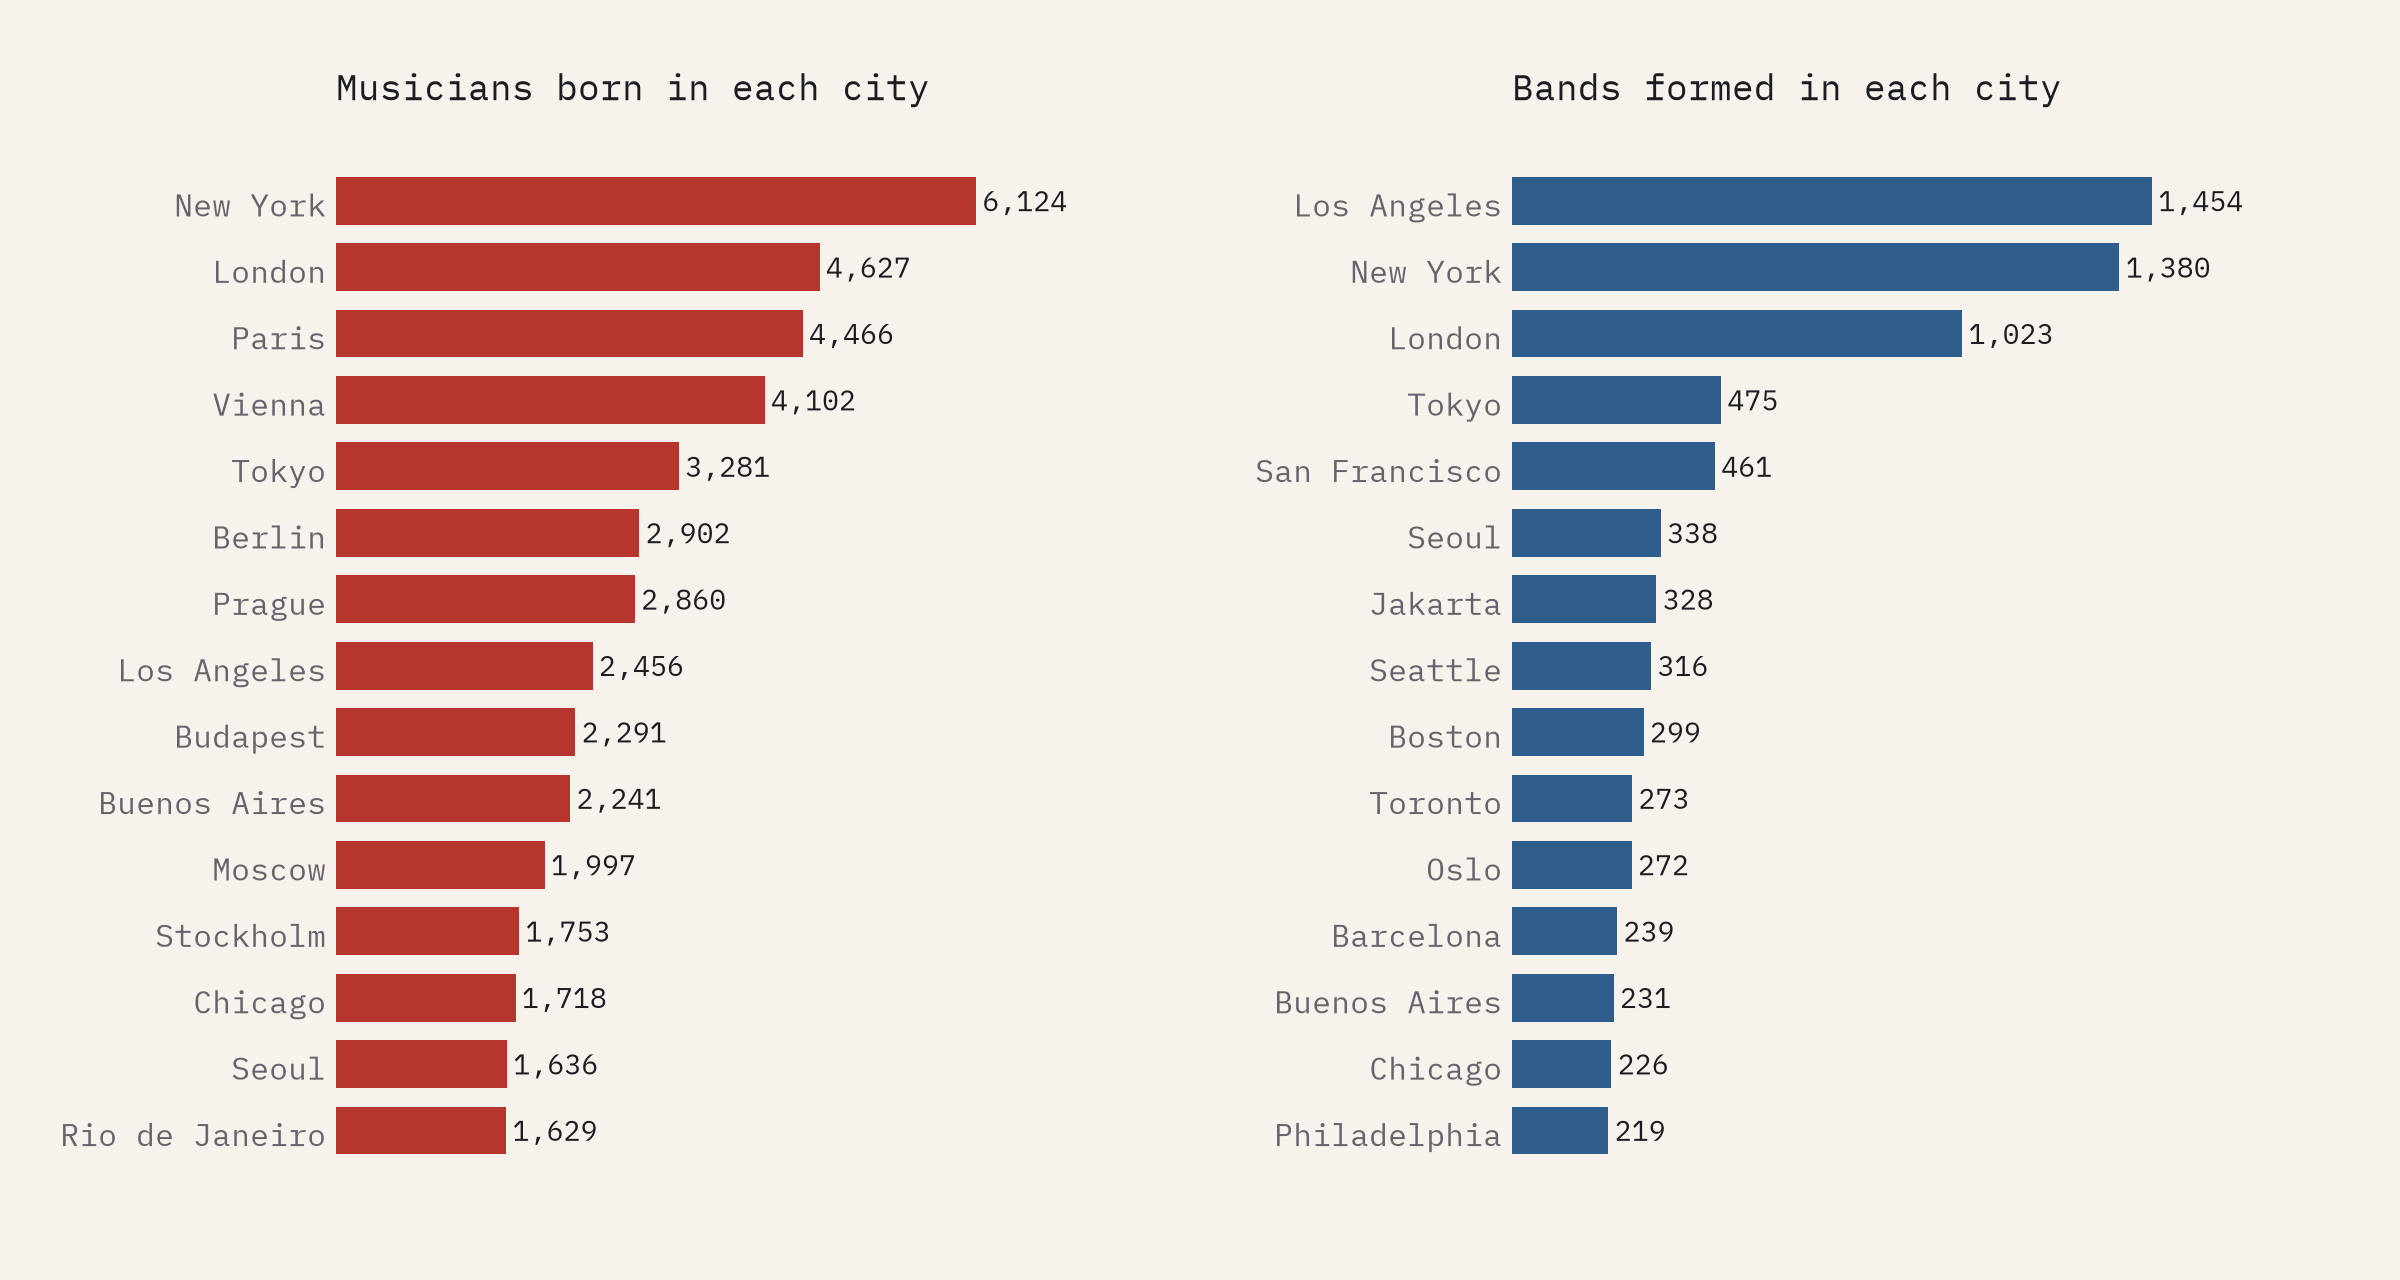
\includegraphics[width=\textwidth]{f_cities.png}
\caption{City areas (points within 25 km of a city of 200,000 or more) with most musicians born and most bands formed.}\label{fig:cities}\end{figure}

\begin{table}[tbp]\centering\small\caption{City areas: most musicians born (with notable musicians), most musicians per 100,000 present-day residents (cities with 150+ musicians), and most bands formed.}\label{tab:cities}\setlength{\tabcolsep}{5pt}\begin{tabular}{lrr@{\hspace{14pt}}lr@{\hspace{14pt}}lr}\toprule City & Musicians & Notable & City & Per 100,000 & City & Bands\\\midrule
New York & 6,124 & 636 & Tallinn & 253.5 & Los Angeles & 1,454\\
London & 4,627 & 426 & Prague & 246.1 & New York & 1,380\\
Paris & 4,466 & 227 & Brno & 244.7 & London & 1,023\\
Vienna & 4,102 & 83 & Erfurt & 234.7 & Tokyo & 475\\
Tokyo & 3,281 & 81 & Trieste & 180.5 & San Francisco & 461\\
Berlin & 2,902 & 74 & San Sebastián & 177.6 & Seoul & 338\\
Prague & 2,860 & 40 & Ljubljana & 175.0 & Jakarta & 328\\
Los Angeles & 2,456 & 320 & Vienna & 170.9 & Seattle & 316\\
Budapest & 2,291 & 43 & Graz & 167.9 & Boston & 299\\
Buenos Aires & 2,241 & 37 & Salzburg & 164.8 & Toronto & 273\\
Moscow & 1,997 & 81 & Dresden & 152.9 & Oslo & 272\\
Stockholm & 1,753 & 70 & Amsterdam & 148.3 & Barcelona & 239\\
Chicago & 1,718 & 135 & Leipzig & 142.1 & Buenos Aires & 231\\
Seoul & 1,636 & 152 & Pisa & 140.2 & Chicago & 226\\
Rio de Janeiro & 1,629 & 31 & Bergen & 139.5 & Philadelphia & 219\\
\bottomrule\end{tabular}\end{table}

\subsection{Composers' Europe and the popular music world}
The kinds of musician have different maps (Table~\ref{tab:fam}). Conductors and bandleaders (80\% European), instrumentalists and composers are overwhelmingly European; rappers (38\% North American) and songwriters are as often North American as European, and singers are the most Asian family (20\%). Composers born before 1900 (26,083 with a point) were 87.7\% European, led by Vienna (850), Paris (829), London, Prague, Berlin, Naples and Barcelona; pop, rock and metal musicians born in 1940 or later (24,811) were 48.4\% European and 27.0\% North American, led by London, New York and Los Angeles (Figure~\ref{fig:contrast}).

\begin{figure}[tbp]\centering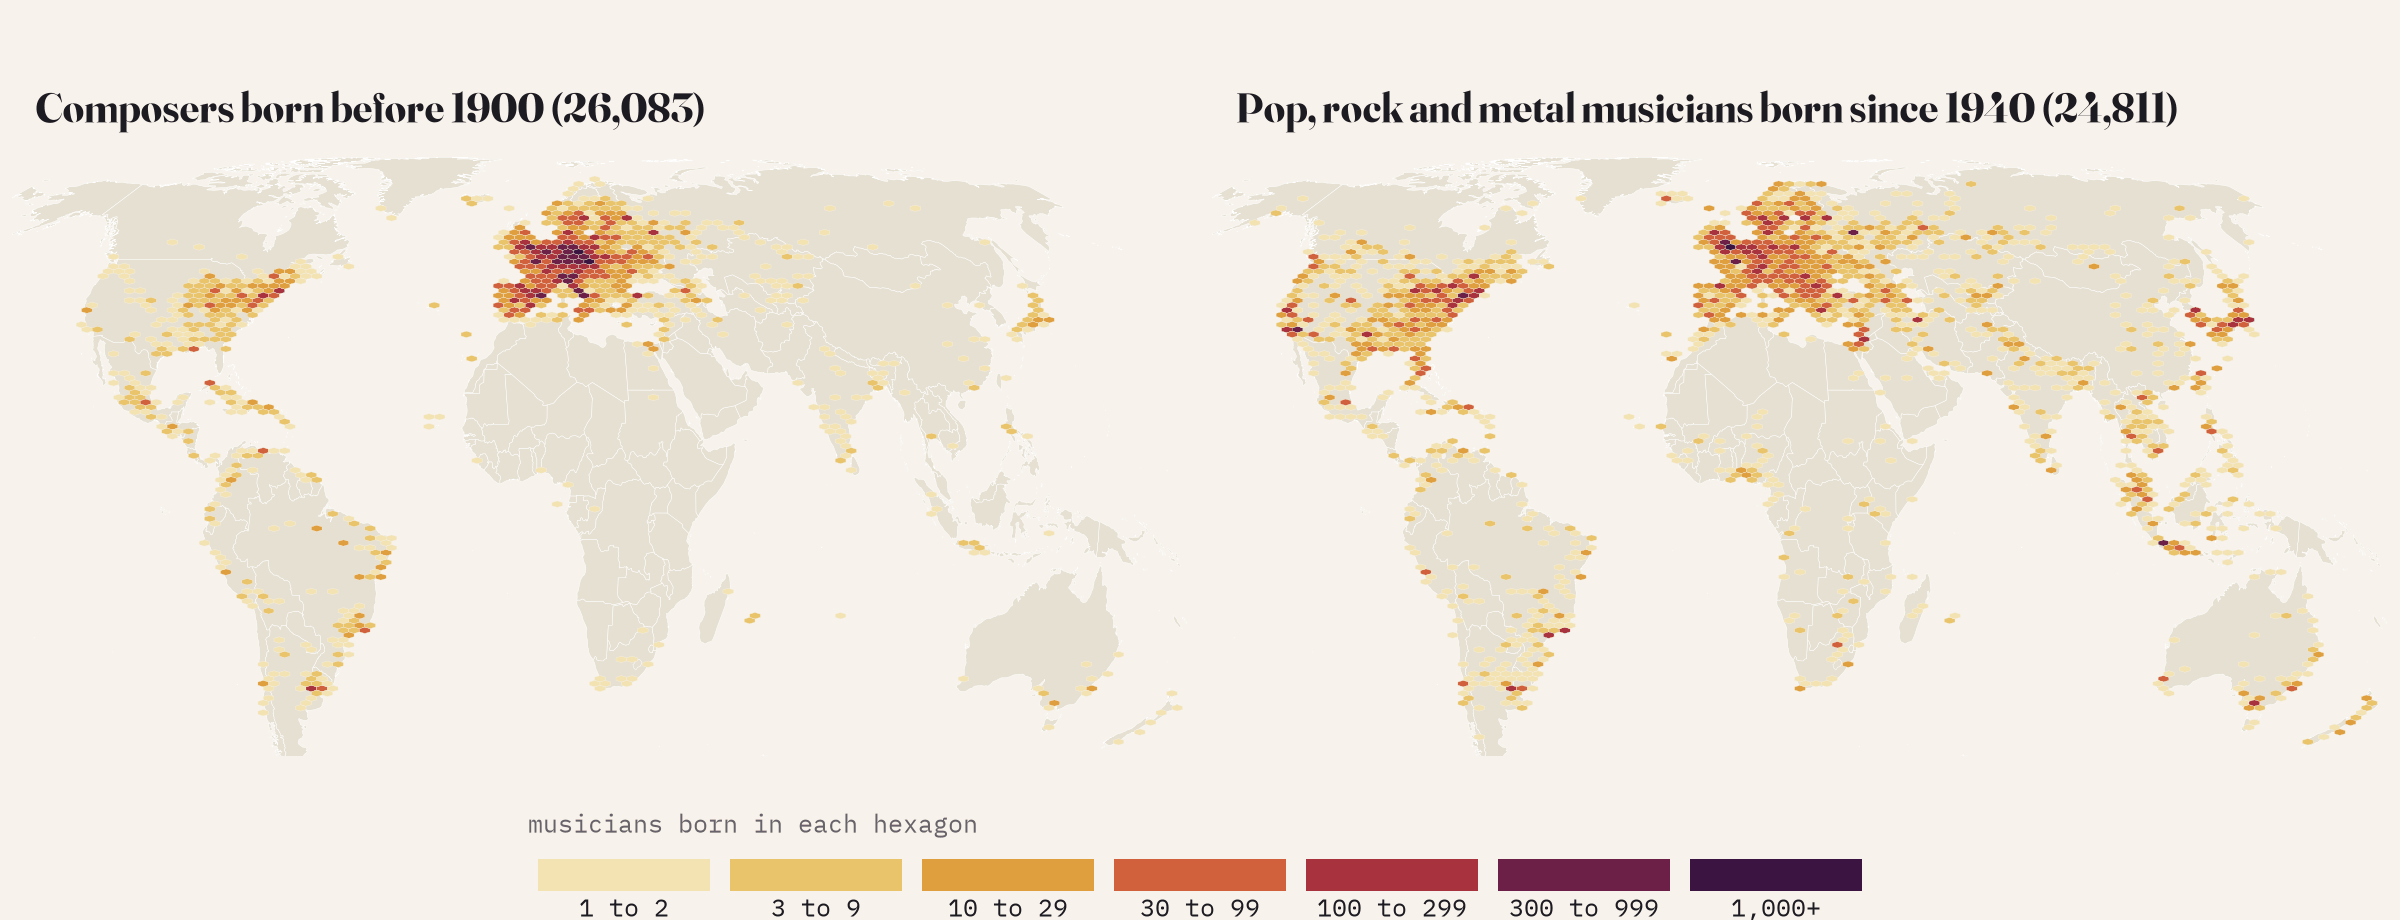
\includegraphics[width=\textwidth]{f_contrast.png}
\caption{Birthplaces of composers born before 1900 and of pop, rock and metal musicians born in 1940 or later.}\label{fig:contrast}\end{figure}

\begin{table}[tbp]\centering\small\caption{Kinds of musician: people in each family (a person can be in several), women's share, and continent of birth.}\label{tab:fam}\setlength{\tabcolsep}{4pt}\begin{tabular}{lrrrrrrr}\toprule Family & People & Women & Europe & N. America & Asia & S. America & Africa\\\midrule
Composers and arrangers & 138,377 & 12.0\% & 65.5\% & 16.2\% & 9.6\% & 6.6\% & 1.4\%\\
Singers & 162,850 & 45.7\% & 51.7\% & 18.1\% & 20.2\% & 5.1\% & 3.7\%\\
Instrumentalists & 117,378 & 16.8\% & 66.8\% & 19.9\% & 7.4\% & 4.2\% & 1.0\%\\
Rappers and MCs & 12,235 & 11.1\% & 36.9\% & 38.3\% & 12.7\% & 3.4\% & 8.2\%\\
DJs and producers & 27,484 & 9.4\% & 46.0\% & 31.8\% & 13.3\% & 4.1\% & 3.6\%\\
Conductors and bandleaders & 35,075 & 7.2\% & 80.0\% & 11.7\% & 4.6\% & 2.7\% & 0.6\%\\
Songwriters & 50,384 & 27.2\% & 38.7\% & 37.5\% & 14.0\% & 3.5\% & 4.6\%\\
Other musicians & 170,393 & 19.6\% & 62.0\% & 22.4\% & 8.1\% & 4.2\% & 2.4\%\\
\bottomrule\end{tabular}\end{table}

\subsection{The home towns of genres}
Most genres are spread across many cities, but several have a clear centre (Figure~\ref{fig:genres}, Table~\ref{tab:sig}). Cantopop is concentrated in Hong Kong (74\% of its acts), samba in Rio de Janeiro (57\%), grime in London (56\%), tango in Buenos Aires (52\%), K-pop in Seoul (52\%) and fado in Lisbon (49\%); reggae and dancehall in Kingston, Afrobeats in Lagos, grunge in Seattle and black metal in Oslo, with Bergen second. Country music is the exception that proves the measure: its acts are spread across the United States, so Nashville holds only 4.8\% of them, yet Nashville's own acts are 13.0 times as likely as the world's to be country. By the location quotient, reggae and its relatives are most concentrated in Kingston (35.4), jazz in New Orleans (4.5), hip hop in Atlanta (4.8) and soul and R\&B in Lagos and Detroit.

\begin{figure}[tbp]\centering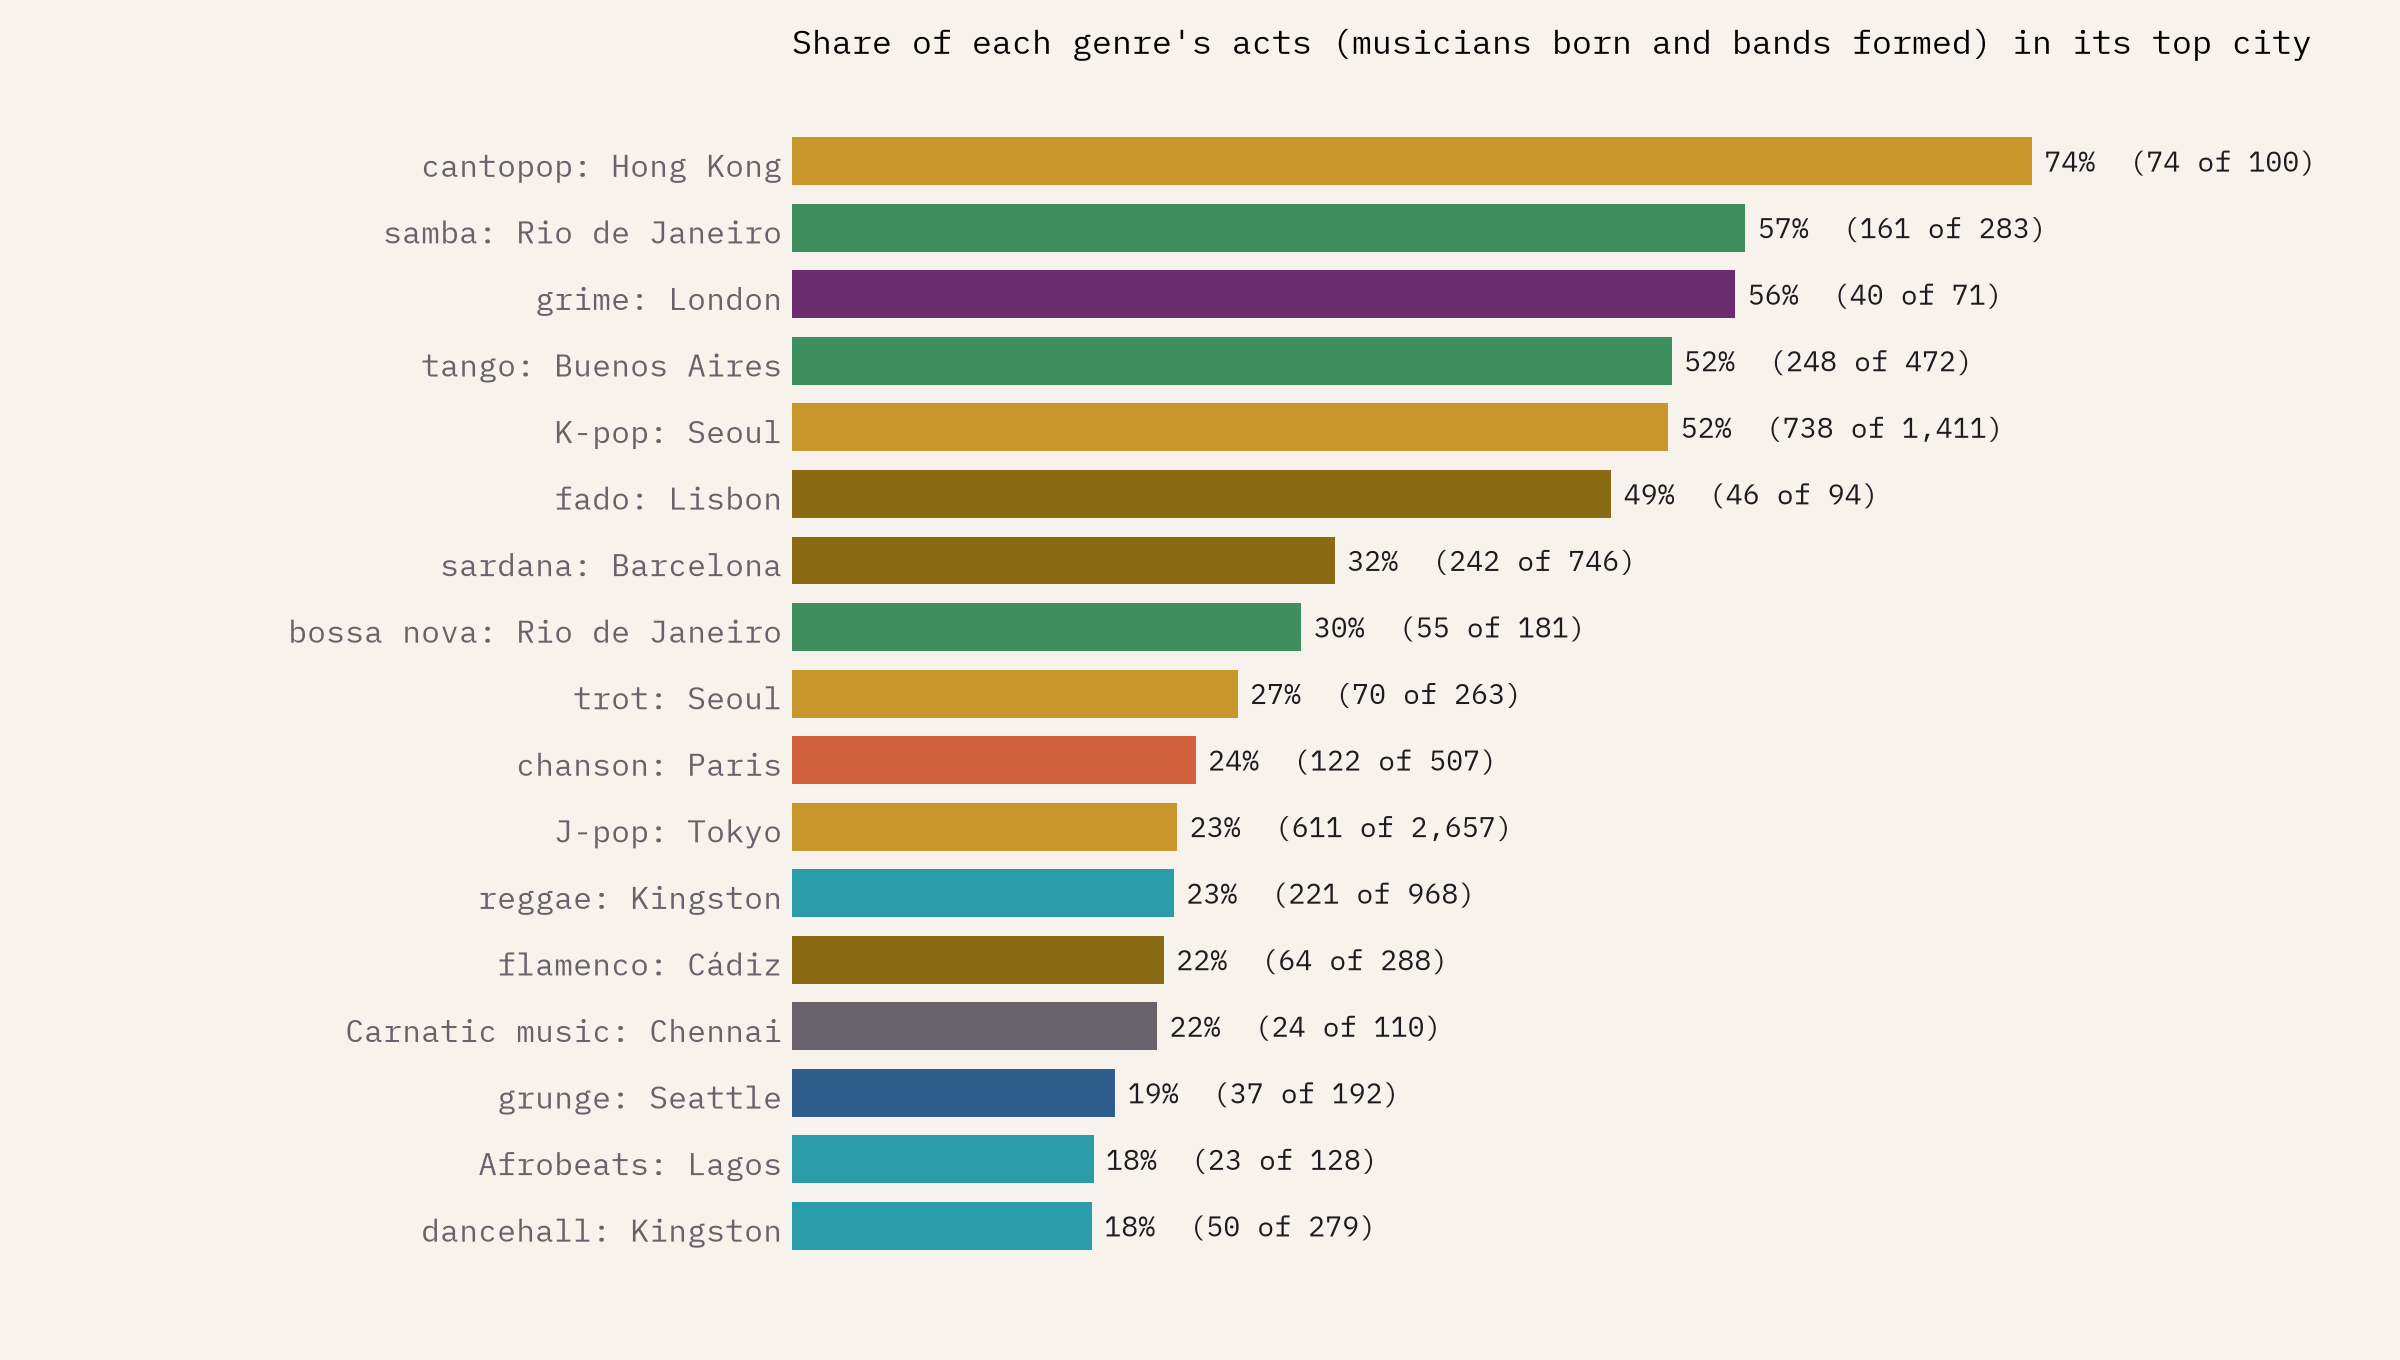
\includegraphics[width=\textwidth]{f_genres.png}
\caption{Share of each genre's acts (musicians born and groups formed, with a point) in the city area with most of them. Genres with 20 or more acts in that city.}\label{fig:genres}\end{figure}

\begin{table}[tbp]\centering\small\caption{Home towns of named genres: the city area with most acts (musicians born and groups formed) tagged with the genre, the number of such acts on the map, the city's share, and the runner-up.}\label{tab:sig}\setlength{\tabcolsep}{5pt}\begin{tabular}{llrrrlr}\toprule Genre & City & Acts & Of & Share & Next & Acts\\\midrule
cantopop & Hong Kong & 74 & 100 & 74.0\% & Shanghai & 3\\
samba & Rio de Janeiro & 161 & 283 & 56.9\% & São Paulo & 25\\
grime & London & 40 & 71 & 56.3\% & Birmingham & 4\\
tango & Buenos Aires & 248 & 472 & 52.5\% & Montevideo & 27\\
K-pop & Seoul & 738 & 1,411 & 52.3\% & Busan & 77\\
fado & Lisbon & 46 & 94 & 48.9\% & Porto & 8\\
sardana & Barcelona & 242 & 746 & 32.4\% & Valencia & 7\\
bossa nova & Rio de Janeiro & 55 & 181 & 30.4\% & São Paulo & 14\\
trot & Seoul & 70 & 263 & 26.6\% & Busan & 26\\
chanson & Paris & 122 & 507 & 24.1\% & Moscow & 16\\
J-pop & Tokyo & 611 & 2,657 & 23.0\% & Ōsaka & 262\\
reggae & Kingston & 221 & 968 & 22.8\% & London & 27\\
flamenco & Cádiz & 64 & 288 & 22.2\% & Seville & 29\\
Carnatic music & Chennai & 24 & 110 & 21.8\% & Mumbai & 5\\
grunge & Seattle & 37 & 192 & 19.3\% & Los Angeles & 8\\
Afrobeats & Lagos & 23 & 128 & 18.0\% & Port Harcourt & 4\\
dancehall & Kingston & 50 & 279 & 17.9\% & London & 9\\
reggaeton & San Juan & 73 & 412 & 17.7\% & Lima & 26\\
salsa & New York & 30 & 179 & 16.8\% & Lima & 27\\
highlife & Accra & 7 & 49 & 14.3\% & Lagos & 6\\
sertanejo & São Paulo & 13 & 106 & 12.3\% & Goiânia & 8\\
Britpop & London & 11 & 92 & 12.0\% & Liverpool & 7\\
house music & New York & 63 & 707 & 8.9\% & Chicago & 47\\
black metal & Oslo & 38 & 500 & 7.6\% & Bergen & 20\\
jazz & New York & 808 & 11,580 & 7.0\% & Chicago & 278\\
schlager & Berlin & 31 & 462 & 6.7\% & Helsinki & 16\\
techno & London & 20 & 348 & 5.7\% & Detroit & 17\\
heavy metal & Los Angeles & 82 & 1,593 & 5.1\% & New York & 59\\
country music & Nashville & 118 & 2,463 & 4.8\% & New York & 50\\
trap music & New York & 33 & 681 & 4.8\% & Atlanta & 30\\
blues & New York & 60 & 1,535 & 3.9\% & Chicago & 54\\
death metal & Stockholm & 21 & 588 & 3.6\% & Tampa & 18\\
opera & Paris & 169 & 5,045 & 3.3\% & Naples & 88\\
bluegrass & Toronto & 8 & 241 & 3.3\% & Los Angeles & 8\\
\bottomrule\end{tabular}\end{table}

\subsection{Countries and bands per head}
The United States is the birth country of 42,298 musicians (14\%), then Germany (31,200), the United Kingdom, Italy, France, Japan and the Czech Republic (Figure~\ref{fig:countries}). Among notable musicians the United States accounts for 34\% and the United Kingdom is second. Per head the Czech Republic (1,131 per million), Austria and Estonia stand out, which is in large part a sign of systematic import of national library records. For bands, the Nordic countries lead per head (Figure~\ref{fig:metal}): Finland has 553.8 bands in Wikidata per million people, Norway 376.4 and Sweden 266.2, and for metal bands 84.8, 55.5 and 56.2, against 12.3 in Germany and 6.7 in the United States.

\begin{figure}[tbp]\centering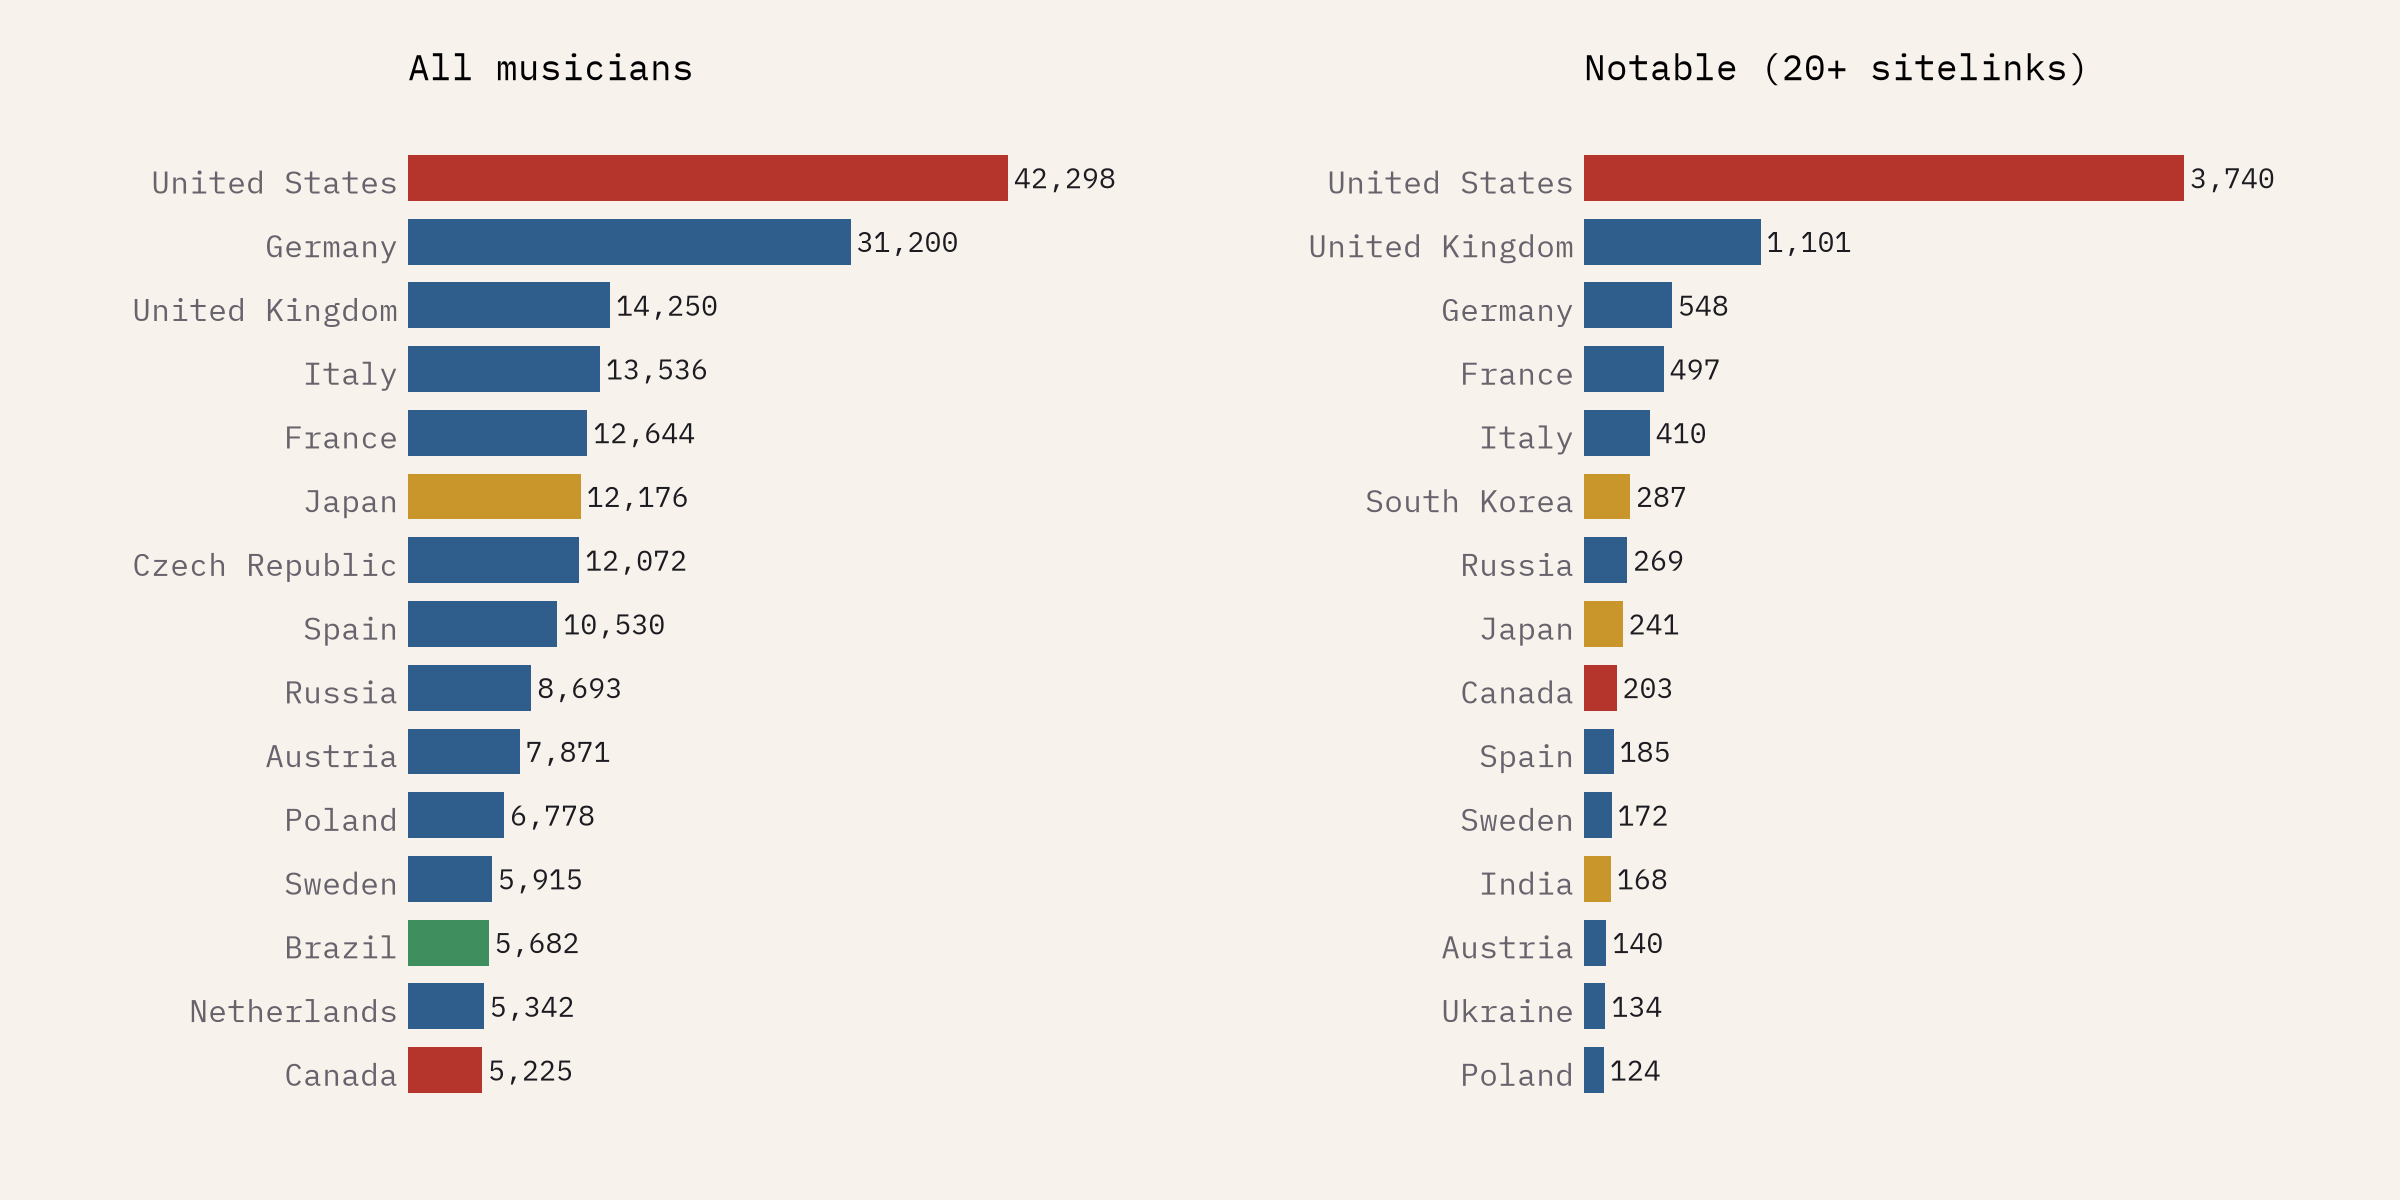
\includegraphics[width=\textwidth]{f_countries.png}
\caption{Musicians by country of birth: all with a birth country, and notable musicians. Colours: continent.}\label{fig:countries}\end{figure}

\begin{figure}[tbp]\centering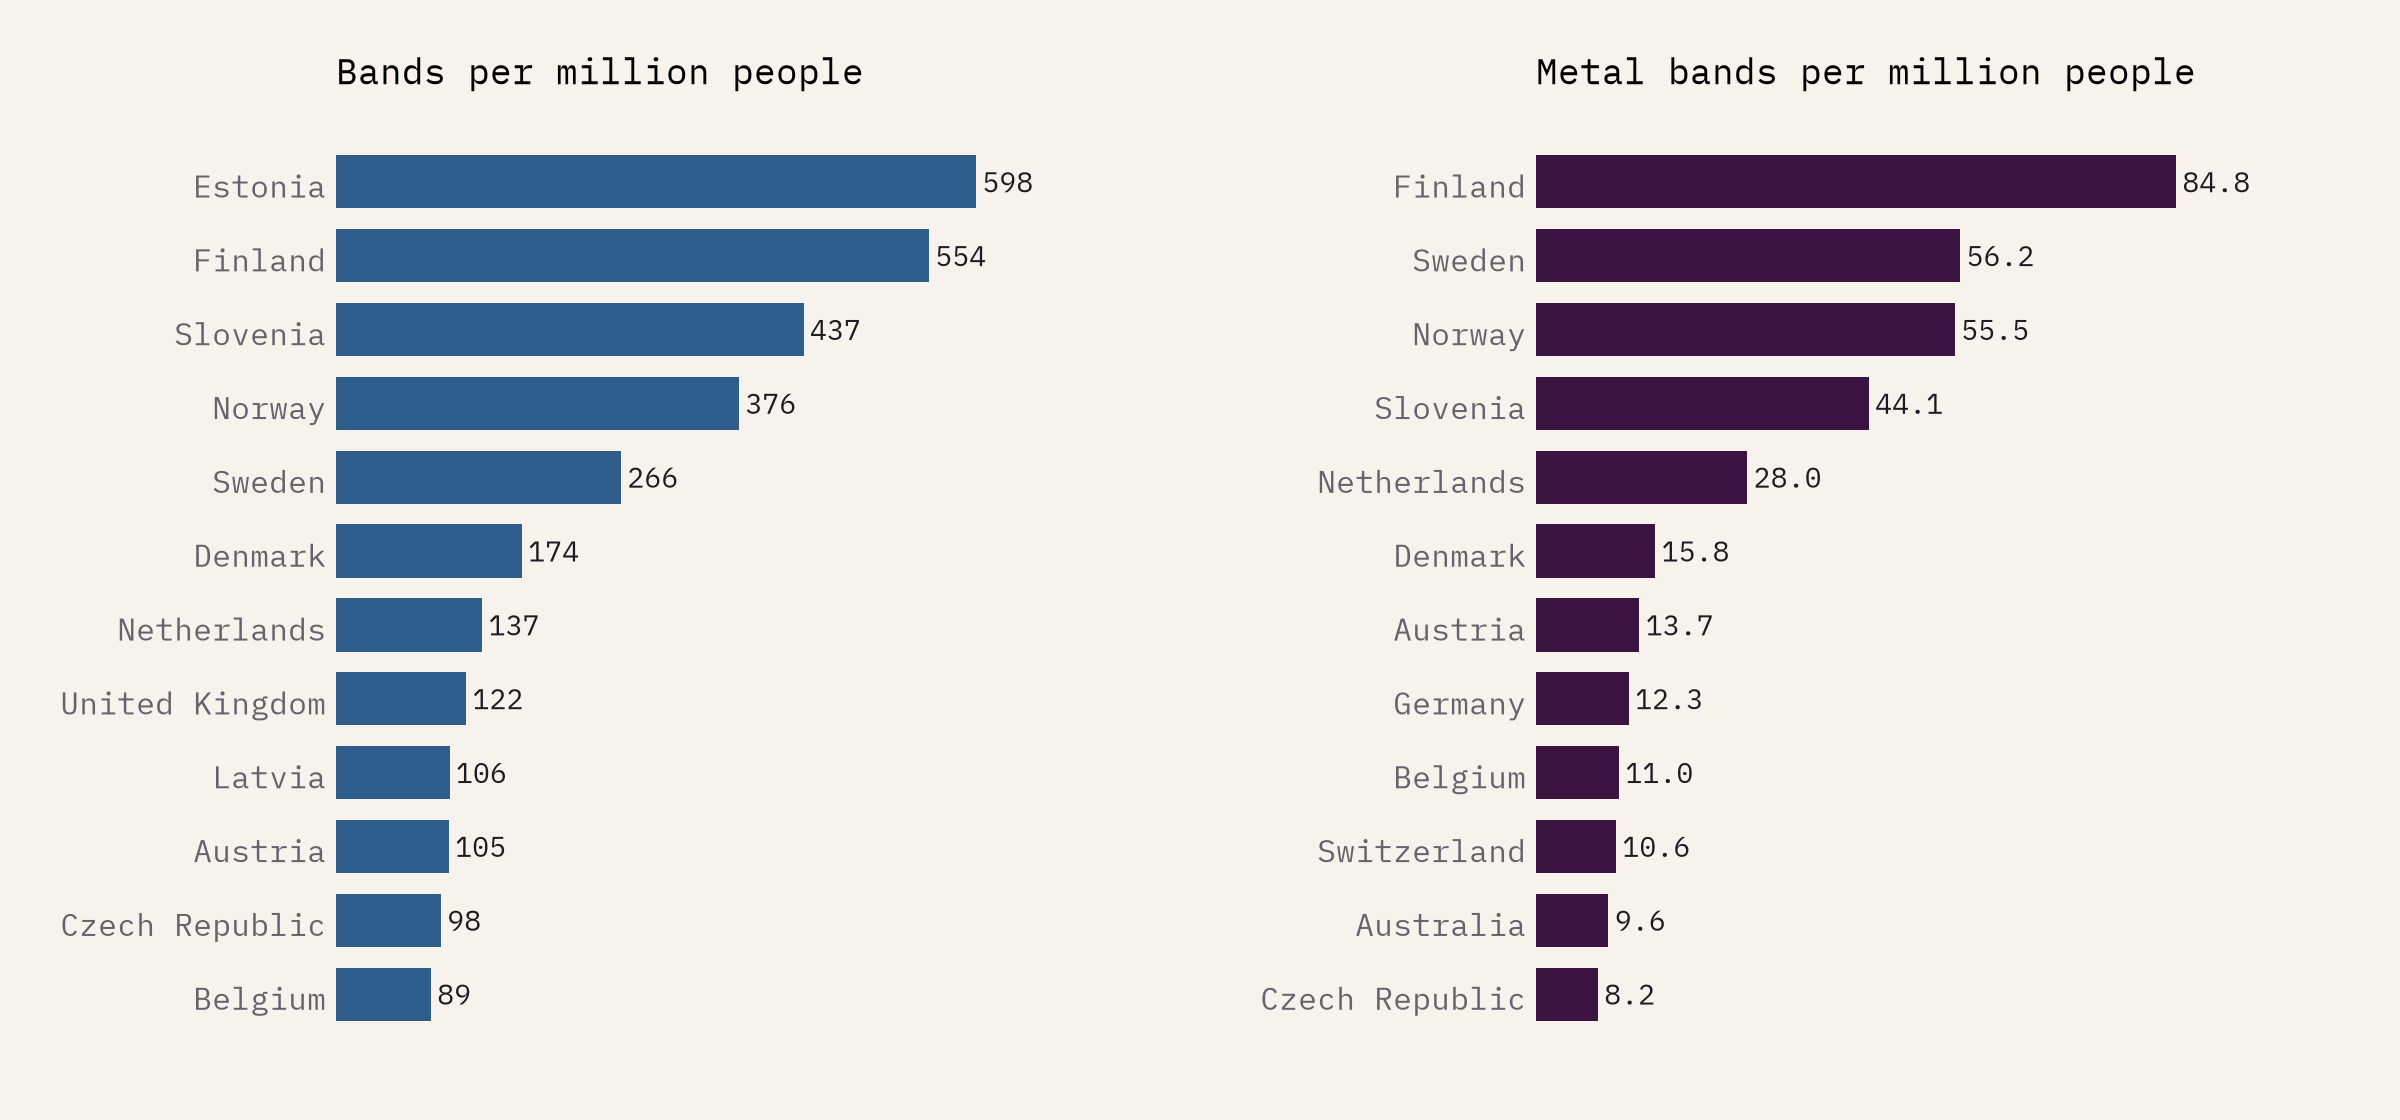
\includegraphics[width=\textwidth]{f_metal.png}
\caption{Bands and metal bands per million present-day population, countries of a million or more with 100+ bands (30+ metal bands).}\label{fig:metal}\end{figure}

\subsection{The shift by decade of birth}
Figure~\ref{fig:shift} shows musicians' continents of birth by decade. Of those born before 1900, 87.2\% were born in Europe and 2.3\% in Asia; of those born since 1970, 49.1\% and 22.7\%. Germany falls from 18.6\% to 8.2\%, Italy from 9.3\% to 3.0\%, while the United States rises from 6.3\% to 14.3\%, Japan from 0.3\% to 6.1\% and South Korea from almost nothing to 3.4\% (Figure~\ref{fig:rise}). Groups are young: 96\% of those with a known start were formed in 1960 or later, most in the 2000s.

\begin{figure}[tbp]\centering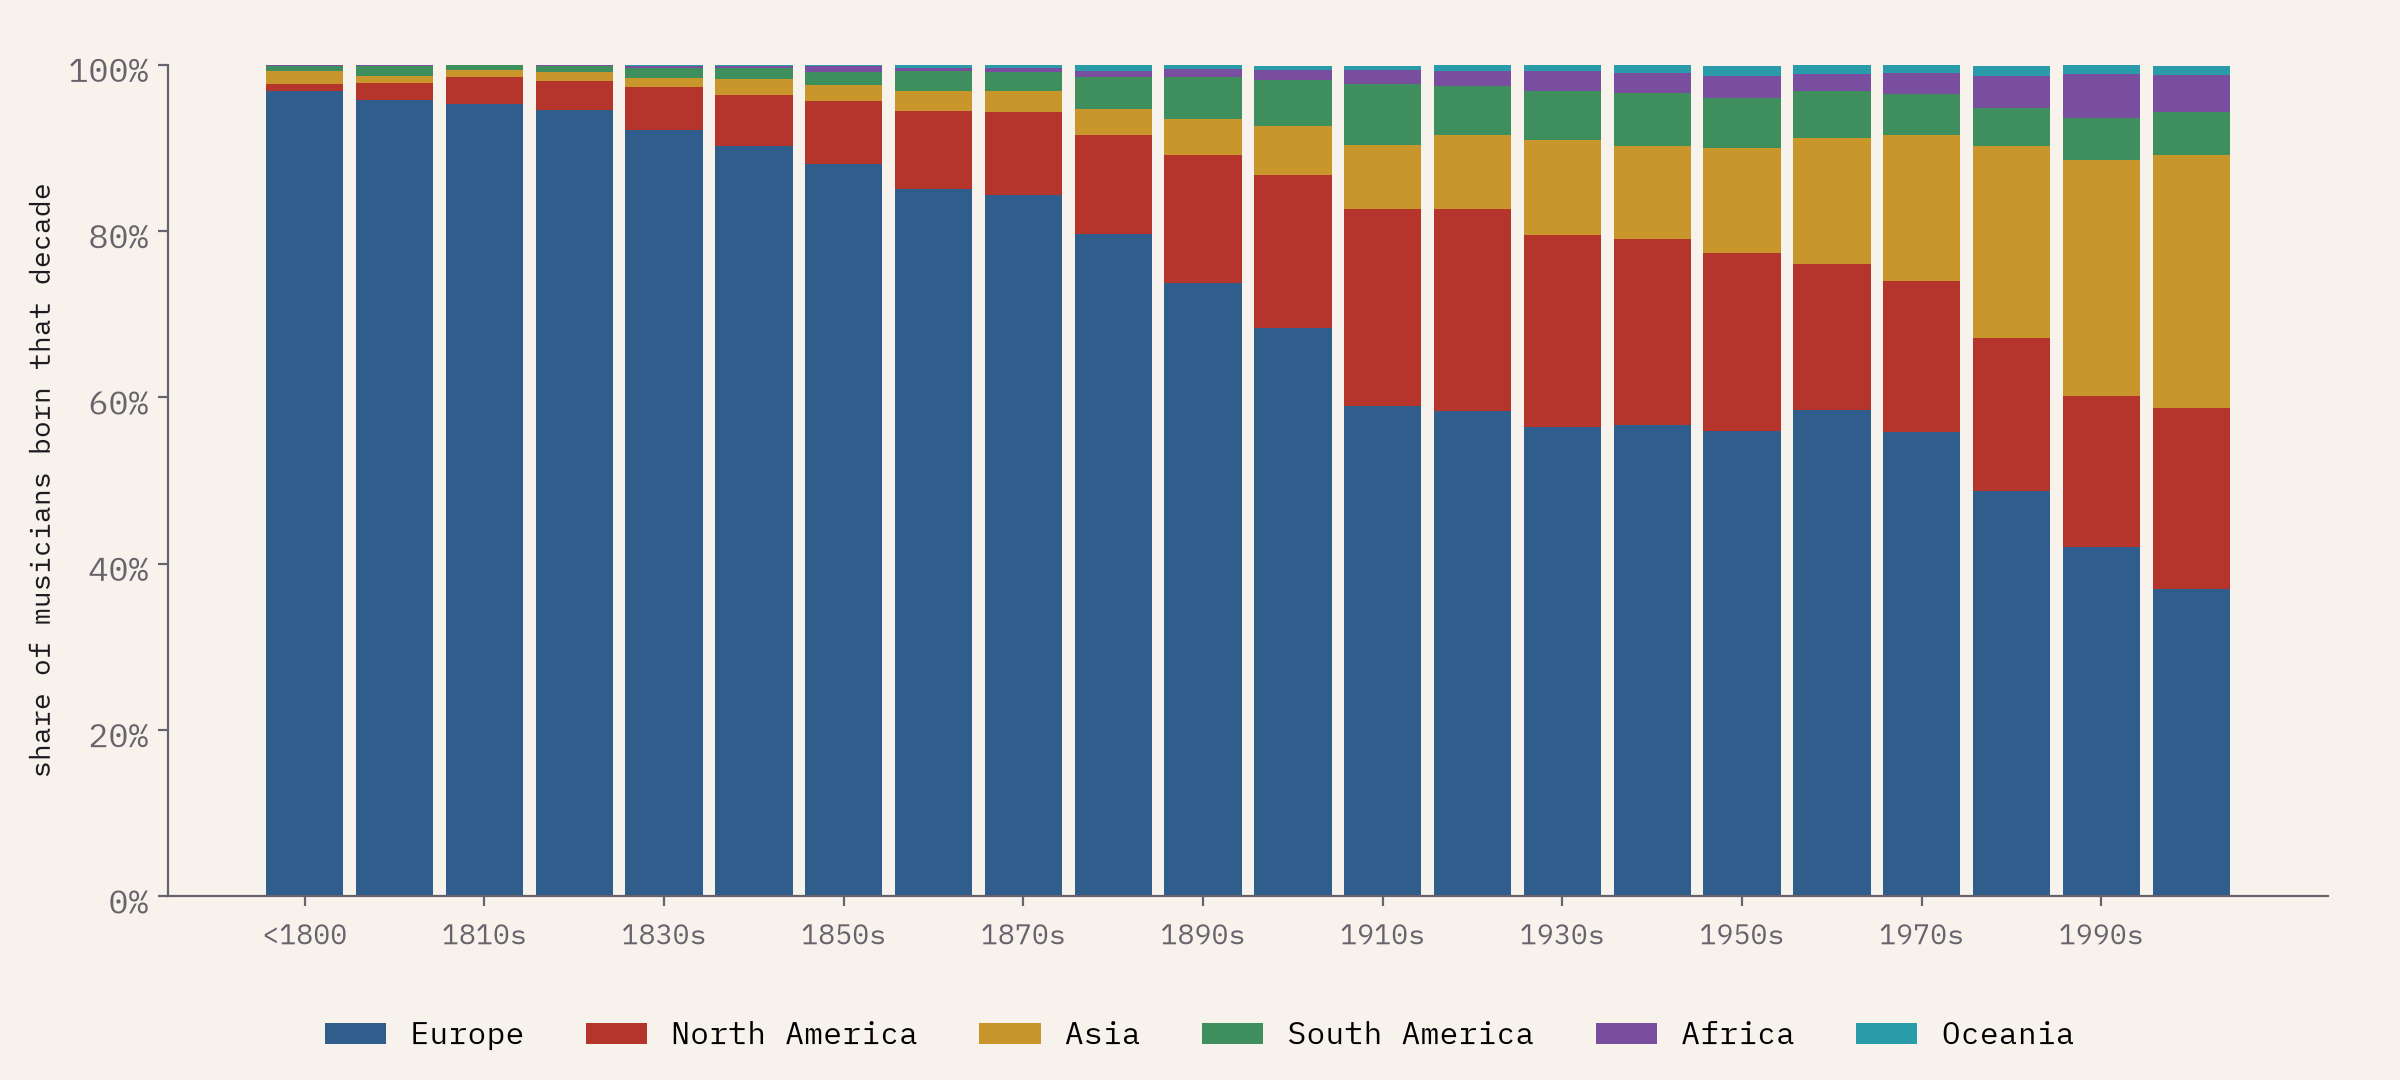
\includegraphics[width=\textwidth]{f_shift.png}
\caption{Continent of birth of musicians, by decade of birth (before 1800 pooled).}\label{fig:shift}\end{figure}

\begin{figure}[tbp]\centering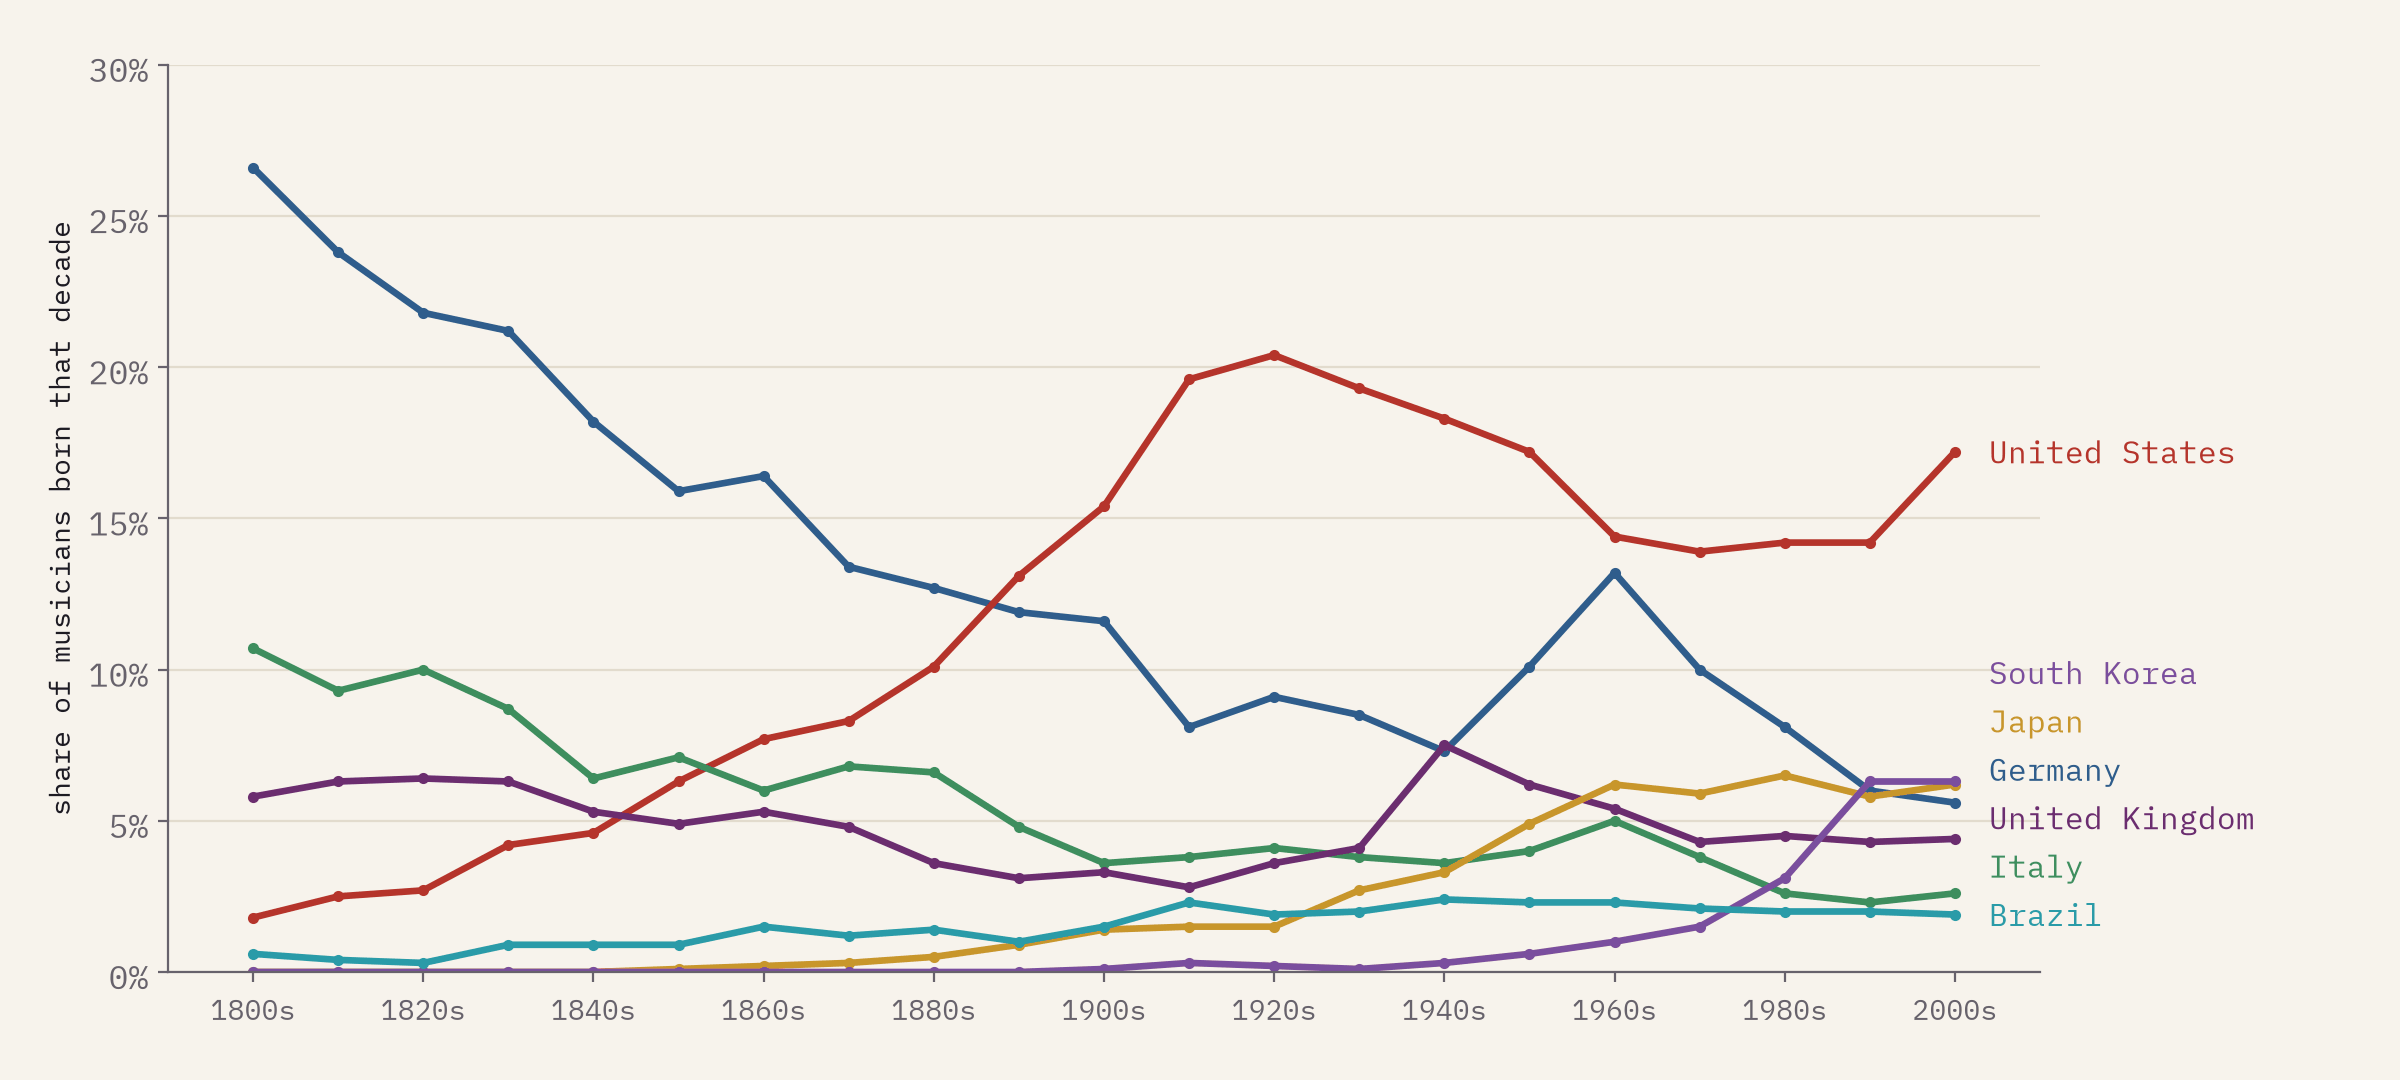
\includegraphics[width=\textwidth]{f_rise.png}
\caption{Share of each decade's musicians born in selected countries.}\label{fig:rise}\end{figure}

\subsection{Women}
Women are 25.4\% of musicians with a recorded gender and 35.4\% of notable ones. By decade of birth (Figure~\ref{fig:women}, Table~\ref{tab:women}) the share rises from 8.1\% before 1800 to about a fifth through the nineteenth century, stays near a fifth for musicians born between 1900 and the 1950s, and then rises to 26.4\% for the 1970s, 36.8\% for the 1980s and 41.9\% for the 1990s. The kind of musician matters more than the decade: women are 45.7\% of singers, 27.2\% of songwriters, 16.8\% of instrumentalists, 12.0\% of composers, 11.1\% of rappers, 9.4\% of DJs and producers and 7.2\% of conductors. Among genre families, East Asian pop has a majority of women (53.8\%) and metal the smallest share (9.0\%). By birth country, the highest shares are for musicians born in Indonesia, China, South Korea and Japan, all above 40\%, and among the lowest for Germany, the Czech Republic and Italy, where catalogues of classical musicians weigh heavily.

\begin{figure}[tbp]\centering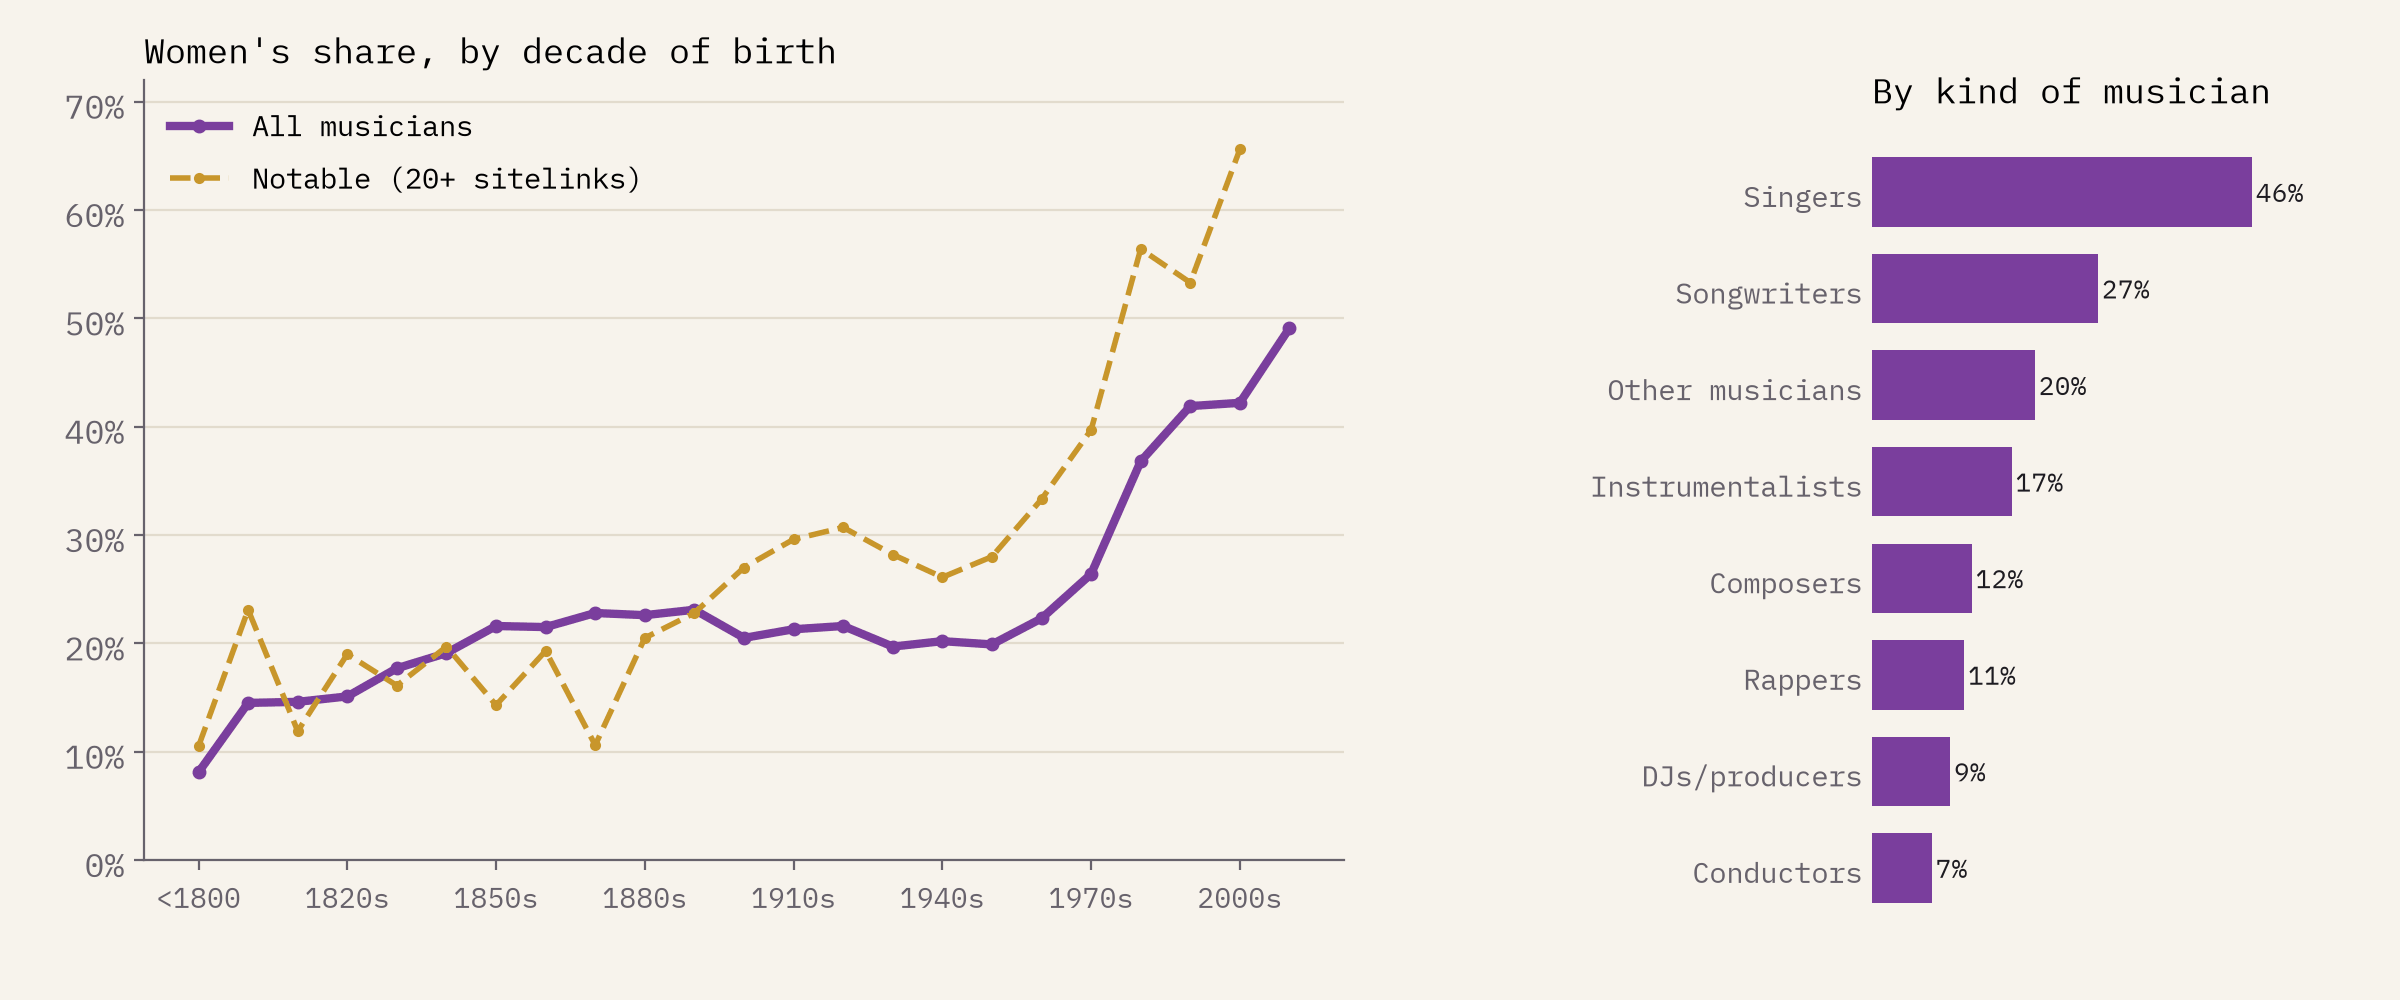
\includegraphics[width=\textwidth]{f_women.png}
\caption{Women's share of musicians by decade of birth, for all and notable musicians, and by kind of musician.}\label{fig:women}\end{figure}

\begin{table}[tbp]\centering\small\caption{By decade of birth: musicians with a recorded gender, women, women's share among all and among notable musicians (where 30 or more), and the share of all musicians with a birth country.}\label{tab:women}\begin{tabular}{lrrrrrr}\toprule Born & With gender & Women & Share & Notable & Share & Birth country known\\\midrule
before 1800 & 16,930 & 1,367 & 8.1\% & 618 & 10.5\% & 68\%\\
1800s & 2,223 & 323 & 14.5\% & 39 & 23.1\% & 73\%\\
1810s & 2,639 & 386 & 14.6\% & 59 & 11.9\% & 75\%\\
1820s & 2,940 & 443 & 15.1\% & 42 & 19.0\% & 76\%\\
1830s & 3,186 & 563 & 17.7\% & 56 & 16.1\% & 78\%\\
1840s & 3,846 & 733 & 19.1\% & 61 & 19.7\% & 78\%\\
1850s & 4,870 & 1,051 & 21.6\% & 56 & 14.3\% & 75\%\\
1860s & 5,994 & 1,289 & 21.5\% & 88 & 19.3\% & 77\%\\
1870s & 7,476 & 1,702 & 22.8\% & 113 & 10.6\% & 77\%\\
1880s & 8,842 & 1,995 & 22.6\% & 161 & 20.5\% & 77\%\\
1890s & 10,153 & 2,349 & 23.1\% & 228 & 22.8\% & 77\%\\
1900s & 15,090 & 3,090 & 20.5\% & 256 & 27.0\% & 73\%\\
1910s & 13,898 & 2,957 & 21.3\% & 358 & 29.6\% & 76\%\\
1920s & 19,228 & 4,154 & 21.6\% & 592 & 30.7\% & 78\%\\
1930s & 22,659 & 4,454 & 19.7\% & 717 & 28.2\% & 76\%\\
1940s & 31,611 & 6,393 & 20.2\% & 1,142 & 26.1\% & 75\%\\
1950s & 39,959 & 7,958 & 19.9\% & 970 & 28.0\% & 71\%\\
1960s & 42,834 & 9,573 & 22.3\% & 1,170 & 33.3\% & 70\%\\
1970s & 46,155 & 12,169 & 26.4\% & 1,380 & 39.7\% & 71\%\\
1980s & 41,610 & 15,307 & 36.8\% & 1,549 & 56.4\% & 72\%\\
1990s & 25,044 & 10,489 & 41.9\% & 1,068 & 53.3\% & 73\%\\
2000s & 9,632 & 4,060 & 42.2\% & 186 & 65.6\% & 62\%\\
2010s & 336 & 165 & 49.1\% & 1 & n/a & 62\%\\
\bottomrule\end{tabular}\end{table}

\subsection{Coverage}
Birthplace coverage is the main limitation (Figure~\ref{fig:cov}). Notable musicians almost always have a birth country (99.8\%); the 61\% of musicians with at most one sitelink only 46\%. Musicians with no date of birth have a birth country only 12.6\% of the time. For groups, a formation place with coordinates is recorded for 25.6\% overall, 17.7\% of those with at most one sitelink and 86.6\% of notable ones. Coverage by kind of musician is more even: among the named kinds it ranges from 61.7\% of DJs and producers to 75.2\% of conductors.

\begin{figure}[tbp]\centering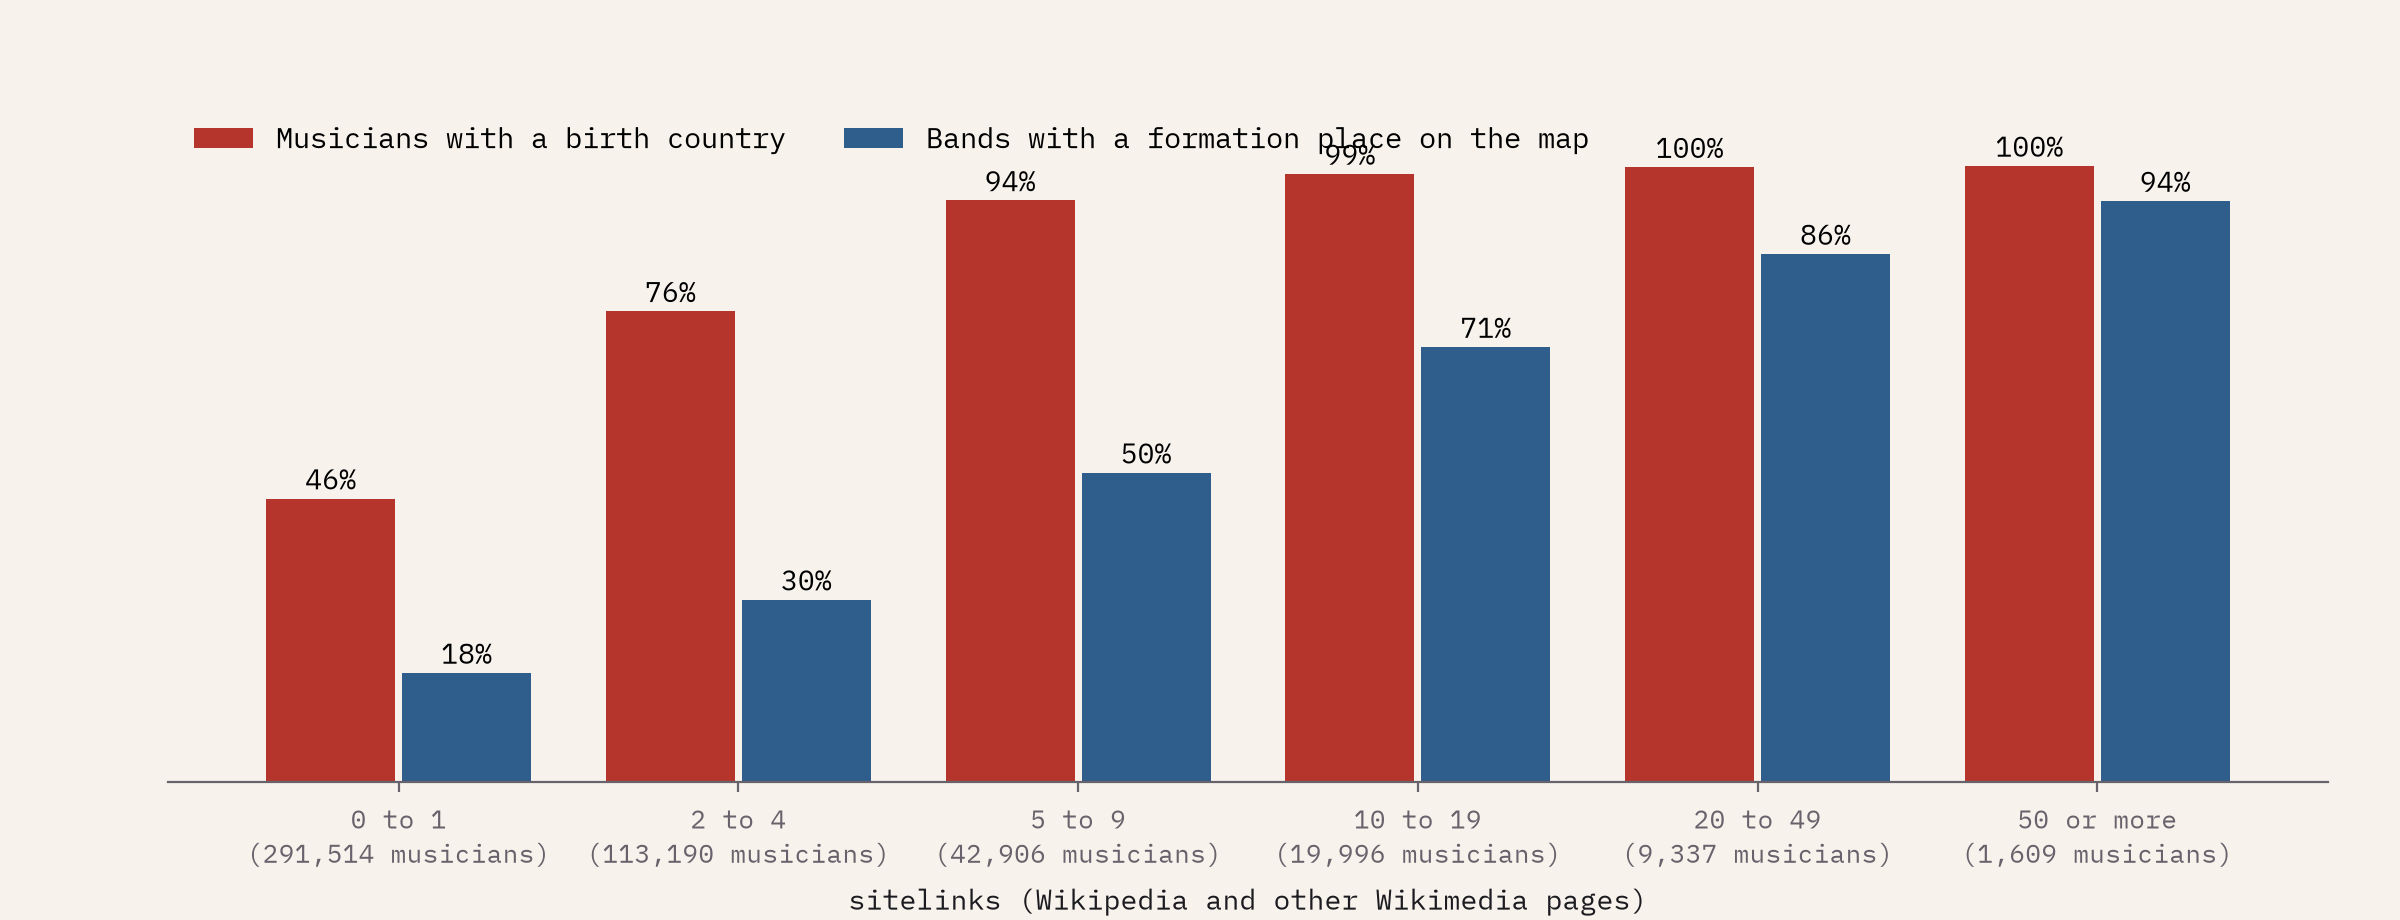
\includegraphics[width=\textwidth]{f_coverage.png}
\caption{Share of musicians with a birth country, and of groups with a formation place on the map, by number of sitelinks.}\label{fig:cov}\end{figure}

\section{Discussion}
The open record reproduces several familiar features of music history: the central European heartland of art music, with Vienna, Paris, Prague and Berlin; the Anglo-American centre of popular music in London, New York and Los Angeles; the rise of Japanese and Korean popular music; and the strong identity of scenes such as Nashville, Kingston, Rio de Janeiro, Buenos Aires, Seattle and Oslo, which the location quotient picks out with no prior knowledge. It also makes visible things that national histories rarely show side by side, such as how much more European conductors are than rappers, or how much more Nordic the band map is than the map of musicians.

Every one of these findings is shaped by coverage. A country's number of musicians in Wikidata depends on whether its national library or music databases have been imported, and whether the import included birthplaces; Tallinn's, Prague's and Brno's high per-head rates are in large part facts about the record. Bands have formation places much less often than musicians have birthplaces, and genre tags are present for a minority of musicians. The safest comparisons are relative ones within the data, such as women's share by kind of musician, or a city's share of a genre's acts.

\section{Limitations}
First, Wikidata is incomplete and uneven: 61\% of musicians have a birth country and 27\% of groups a formation place. Second, the population is defined by Wikidata's occupation classes, which are generous: the most linked `musicians' include Leonardo da Vinci, Goethe, Martin Luther and Nietzsche, who did play or compose. Third, birth countries use present-day borders. Fourth, families of occupations and genres come from rules on English labels; a few assignments are debatable, and the lists are published so readers can regroup them. Fifth, gender is as recorded, mostly binary, and missing for 4\% of musicians. Sixth, city areas use a fixed 25 km radius and present-day populations. Finally, all counts are for one retrieval in 2026.

\section{Conclusion}
A few open queries are enough to map where nearly half a million musicians were born and where tens of thousands of bands formed, to show how that geography moved from central Europe towards North America and East Asia, to find the home towns of genres, and to measure how unevenly women appear across kinds of musician. The same data show clearly where the record is thin. The atlas lets readers explore both.

\section*{Data and code availability}
The interactive atlas is at \url{https://maps.tristanhotham.com/music-birthplaces/}. Data and code are at \url{https://github.com/Tristan-Hotham/music-birthplaces} and archived with this paper at https://doi.org/10.5281/zenodo.23850287. Derived data are released under CC BY 4.0 and code under the MIT licence.

\section*{AI statement}
I wrote the text, with drafting and editing assistance from Claude (Anthropic), which also helped prepare the analysis code. I reviewed and checked all text and results.

\begin{thebibliography}{9}
\bibitem[Bast and Buchhold(2017)]{qlever} Bast, H. and Buchhold, B. (2017) QLever: a query engine for efficient SPARQL+text search. \emph{Proceedings of the 2017 ACM Conference on Information and Knowledge Management}, 647 to 656.
\bibitem[Bennett and Peterson(2004)]{bennett} Bennett, A. and Peterson, R. A. (eds.) (2004) \emph{Music Scenes: Local, Translocal and Virtual}. Nashville: Vanderbilt University Press.
\bibitem[Carney(1974)]{carney} Carney, G. O. (1974) Bluegrass grows all around: the spatial dimensions of a country music style. \emph{Journal of Geography}, 73(4), 34 to 55.
\bibitem[Connell and Gibson(2003)]{connell} Connell, J. and Gibson, C. (2003) \emph{Sound Tracks: Popular Music, Identity and Place}. London: Routledge.
\bibitem[Natural Earth(2026)]{naturalearth} Natural Earth (2026) Admin 0 countries, land and populated places. Public domain. \url{https://www.naturalearthdata.com/}
\bibitem[Schich et al.(2014)]{schich} Schich, M., Song, C., Ahn, Y.-Y., Mirsky, A., Martino, M., Barab\'asi, A.-L. and Helbing, D. (2014) A network framework of cultural history. \emph{Science}, 345(6196), 558 to 562.
\bibitem[Vrandečić and Krötzsch(2014)]{wikidata} Vrandečić, D. and Krötzsch, M. (2014) Wikidata: a free collaborative knowledgebase. \emph{Communications of the ACM}, 57(10), 78 to 85.
\bibitem[Wagner et al.(2016)]{wagner} Wagner, C., Graells-Garrido, E., Garcia, D. and Menczer, F. (2016) Women through the glass ceiling: gender asymmetries in Wikipedia. \emph{EPJ Data Science}, 5, 5.
\end{thebibliography}
\end{document}
